%style
\documentclass[12pt]{article}
%\usepackage{eurosym}
\usepackage[top=1in, bottom=1in, left=1in, right=1in]{geometry}
\usepackage{fancyhdr}

%packages
\usepackage{adjustbox}
\usepackage{amsmath}
\usepackage{amssymb}
\usepackage{array}
\usepackage{bm}
\usepackage{bbold}
\usepackage{booktabs}
%\usepackage{float}
\usepackage{graphicx}
\usepackage[colorlinks=true,linkcolor=blue,urlcolor=blue,anchorcolor=blue,citecolor=blue]{hyperref}
\usepackage{lscape}
\usepackage{multirow}
\usepackage{natbib}
\usepackage{setspace}
\usepackage{tabularx}
\usepackage[titletoc]{appendix}
\usepackage{pgffor}

\usepackage[table]{xcolor}
\usepackage{tabu}
\usepackage{makecell}
\usepackage{longtable}
\usepackage{multirow}
\usepackage[normalem]{ulem}
\usepackage{etoolbox}
\usepackage{ragged2e}
\usepackage{fixltx2e}
\usepackage[para, flushleft]{threeparttablex}
\usepackage[capposition=top]{floatrow}
\usepackage{subcaption}
\usepackage{pdfpages}
\usepackage{pdflscape}
\usepackage{bibunits}
\usepackage{marvosym}
\usepackage{makeidx}
\usepackage{tikz}
\usetikzlibrary{shapes}
\usepackage{enumerate}
\usepackage{rotating}
\usepackage{epstopdf}
\usepackage{framed}
\usepackage{comment}
\usepackage{xr}
\usepackage{titlesec}
\usepackage{footnote}
\newlength{\tablewidth}
\setlength{\tablewidth}{9.3in}
\setcounter{secnumdepth}{4}
\usepackage[T1]{fontenc}
\usepackage{calc}


\setcounter{MaxMatrixCols}{10}

%Functions
\DeclareMathOperator{\cov}{Cov}
\DeclareMathOperator{\var}{Var}
\DeclareMathOperator{\plim}{plim}
\DeclareMathOperator*{\argmin}{arg\,min}
\DeclareMathOperator*{\argmax}{arg\,max}

\parindent 22pt
\newcommand{\indep}{\rotatebox[origin=c]{90}{$\models$}}
\newcommand{\mr}{\multirow}
\newcommand{\mc}{\multicolumn}

\newcolumntype{L}[1]{>{\raggedright\let\newline\\\arraybackslash\hspace{0pt}}m{#1}}
\newcolumntype{C}[1]{>{\centering\let\newline\\\arraybackslash\hspace{0pt}}m{#1}}
\newcolumntype{R}[1]{>{\raggedleft\let\newline\\\arraybackslash\hspace{0pt}}m{#1}}

\definecolor{maroon}{HTML}{990012}


\begin{document}

\title{Analysis of the Reggio Approach} %Evaluating the impact of high quality infant-toddler centers and preschools in northern Italy
\author{Pietro Biroli, Daniela Del Boca, and Chiara Pronzato}
\date{[{\color{red}{VERY PRELIMINARY DRAFT, DO NOT CIRCULATE}}] \\
Original version: January 22, 2016 \\
Current version: \today }

\maketitle

\abstract{A growing literature establishes that providing enriched early environments to children has substantial long-run impacts on a variety of social, economic and health outcomes, with stronger effects for more disadvantaged children. While the impacts are sizable and long-lasting for small-scale randomized controlled trials, it is unclear whether the results can be sustained when brought up to scale. In this paper we evaluate an influential and long-established preschool program, the Reggio Approach to Early Childhood Education. This is a unique natural experiment which has been in place for fifty years in the city of Reggio Emilia, Italy. Here a universal high-quality early child care system has developed a different vision of the child -- as an individual with rights and potential. The Reggio Approach has received world-wide recognition and has been emulated in different countries and in a variety of settings, but it has never been evaluated. We evaluate the short, medium, and long term effects of this programs using newly collected data of children, adolescents, and adults in three cities in northern Italy: Reggio Emilia, Parma, and Padova. Comparing the Reggio Approach to other existing infant-toddler centers and preschools in these cities, we find moderate effects in the domains of sociability and healthy behaviors.}


\bigskip

\doublespacing

\section{Introduction}\label{sec:intro}

This paper aims to evaluate the Reggio Approach preschool system. The Reggio Approach includes infant-toddler centers (ages 0-3) and preschools (ages 3-6), both of which are for children before they enter primary school at age 6. The Reggio infant-toddler center has a long history: it was established in 1971, while the first Reggio preschool was established even earlier, in 1963.

The Reggio Approach (RA) is a unique natural experiment which has been in place for fifty years in the city of Reggio Emilia, Italy. Here a universal high-quality early childcare system has developed a more progressive vision of the child as an individual with rights and potential (\cite{Malaguzzi1993}). The Reggio Approach has received world-wide recognition and was defined as an exemplary model of early childhood education by Newsweek in 1971. It has received over the years several prizes and has been emulated in different countries,\footnote{The official \href{http://www.reggiochildren.it/network/?lang=en}{Reggio Children International Network} is present in 33 countries worldwide. Many other preschools around the world are ``inspired'' by the Reggio Approach but they are not officially part of these network.} but it has never been evaluated.

In order to evaluate the Reggio Approach, we have collected data on five age cohorts, three cohorts of adults, one cohort of adolescents, and one cohort of children in their first year of elementary school. The data were collected in Reggio Emilia, Padova, and Parma. Parma and Padova are similar to Reggio Emilia in several dimensions (size, geographic, demographic and socio-economic structure, and fertility dynamics), but do not provide the same type of early childhood education. The schools that follow the Reggio Approach are the municipal infant-toddler centers and preschools in Reggio Emilia. All of the children who attended a municipal infant-toddler center or preschool in Reggio Emilia are considered part of the treated group, since they received the RA intervention. The other types of schools in Reggio Emilia, and all the schools in Parma and Padova (including the municipal schools) did not receive the RA intervention.

Our analysis is limited to children and adolescents, since the important outcomes collected in our survey are quite similar among them; the cognitive and non cognitive outcomes collected in the interviews are very different for the older and the younger cohorts, which makes reasonable to perform a separate analysis between these two groups. Moreover, the children and adolescent cohorts are likely to have experienced similar childcare supply choices. On the other hand, adults have faced very limited choice of formal childcare, since the first experience started in the early sixties in Reggio Emilia and only later in the other two cities. We are currently working on another section of the paper on the adult cohorts.

The evaluation of the Reggio Approach presents several challenges, given the non-experimental nature of the program. The RA preschool system was introduced and grew over the course of several decades; therefore the evaluation strategy has to deal with potential changes in treatment quality over time, lack of well defined control group, and potential spillover effects. This analysis evaluates the RA aiming to address these issues. We consider several groupings of controls to account for differences by region, data collection, socioeconomic factors, and most importantly type of preschool chosen by the families. Different model specifications allow for comparison with various control groups, allowing for a more nuanced understanding of the effects of RA, including the effects both within and between regions and in relation to other types of early education.

The analysis of the different pedagogical approaches characterizing the different schools (municipal, state, religious, and private in Reggio Emilia, Parma, and Padova) indicates that the principles of holistic and child centered approach started in Reggio Emilia are becoming more and more the norm given the Early Childhood Education and Care (ECEC) directives on childcare (\cite{Bennett2012}).

In the next section, we review some of the previous work on the impact of childcare quality and curriculum on child outcomes. A brief description of the RA is provided in Section \ref{sec:RA} while a comparison between Reggio Emilia and the other two cities involved with the data collection is provided in Section \ref{sec:ParmaPadova}. More detail about the data collection, including sample structure and survey design, is given in Section \ref{sec:data}. A simple model of school selection is sketched in Section \ref{sec:model}. The identification strategy and the empirical analysis are discussed in Section \ref{sec:method}. Section (\ref{sec:conclusion}) provides very preliminary conclusions.

\bigskip

\section{The link between childcare quality, curriculum, and child outcomes} \label{sec:lit}

In the last few years economic research has started analyzing the impact of childcare on child outcomes focusing not only on its availability but also its quality and pedagogical philosophies. \cite{Felfe2015a} analyzed German data, using information on the quality of available childcare for children under the age of three. They show that quality is a very important determinant of several child outcomes at the age of 6, particularly of socio-emotional maturity and school readiness. Specifically, teachers' age and education, working hours, and group size have a positive impact on child outcomes. The effects are stronger for children of less educated mothers.

\cite{DattaGupta2010} and \cite{Bernal2011} analyze the role of quality comparing non cognitive outcomes for children in formal (municipal-regulated) preschool and informal family day-care services with those of children cared for by parents. They finds that formal child care does as well as parental care on non-cognitive outcomes and has a more positive effect on children's behavior than informal child care arrangements.

\cite{Bernal2011} using the National Longitudinal Survey of Youth 1979 focuses on single mothers and shows that informal care has significant negative effects on cognitive achievement, especially for children of more educated mothers, while formal center-based care has no adverse effect.

\cite{Love2003} using data from three different contexts in the U.S., Australia, and Israel (Early Head Start; the Sydney Family Development Project; Haifa-NICHD merged data) compare a variety of childcare centers differing in levels of regulation and of staff quality, and provide consistent evidence that the quality of childcare has an important impact on child development. In particular, children from low-income families experience a stronger positive impact of childcare quality on a both cognitive and non-cognitive outcomes.

\cite{Li2013} explore the effects on later outcomes of high-versus low-quality childcare both during infant--toddlerhood and during the preschool years, using data from the National Institute of Child Health and Human Development Study of Early Child Care. They show that quality matters as well as the timing of attendance of high-quality education. Cognitive, language, and other skills were highest in children who experienced high-quality care in both the infant--toddler and preschool periods, somewhat lower in children who experienced high-quality childcare during only one of these periods, and lowest among children who experienced low-quality care during both periods.

Other studies have linked quality with the influence of certain program curricula and pedagogical philosophies on the teaching strategies employed in classrooms, roughly divided into the two main categories of ``child centered'' and ``academic'' approaches. The Reggio Approach is a clear example of a child centered approach, where the teacher is encouraged to become the child's co-learner and collaborator. According to this approach, teachers do not impose a specific curriculum, but facilitate the child's learning by planning activities based on the child's interests, and engaging in the activities alongside the child (\cite{Malaguzzi1993}, \cite{Hewett2001}). In an academic approach, instead, the focus is on acquiring notions related to different subject areas.

Using data from the Pre-K Survey of Beliefs and Practices, \cite{Marcon1999} identifies three different preschool models operating in an urban school district: child centered, academic driven, and a combination of the two. His empirical evidence shows that by the end of preschool, children from child-centered programs have acquired greater competence in social, basic math, and basic verbal skills than their peers in academically-driven preschool environments.

Other studies have compared the long term effects of several pedagogical models. \cite{Miller1984a} analyzes the achievement test and IQ data on low-income black youths who had participated in traditional and more progressive programs in preschool and prekindergarten through ninth and tenth grades. They find long-term positive effects of child-centered learning on school achievement. \cite{Schweinhart1997} have evaluated long term effects (through age 23) of the High/Scope program vs more traditional preschool curriculum models. Their findings show that using a curriculum model based on child-initiated learning activities improves social behavior at a later age. Specifically they found at age 23, compared to the other curriculum groups, the group who has experienced a more traditional curriculum had three times as many felony arrests per person.

The traditional sequential and subject specific approaches are less effective in promoting children's learning in the early years whereas a holistic approach that sustains children's overall development across several domains is more effective as it is supportive of children's learning strategies (\cite{Bennett2012}). As stated by \cite{Bennett2013}: ``The cognitive life of a young child does not match a traditional `subjects' approach. Rather, it is focused on meaning-making -- his/her place in the family; the roles and work of significant adults; forging a personal identity; how to communicate needs and desires; how to interact successfully and make friends; how things work; the change of the season and other remarkable events in the child's environment.'' Recent ECEC recommendations have addressed the childcare quality issue as a necessary condition for the promotion of children's development and personal fulfillment (\cite{EuropeanCommission2011,Council2011}). According to the recent ECEC directives ``Each child is unique and a competent and active learner whose potential needs to be encouraged and supported. Each child is a curious, capable and intelligent individual. The child is a co-creator of knowledge who needs and wants interaction with other children and adults. As citizens of Europe, children have their own rights which include early education and care.''\footnote{See \cite{ChildrenInEurope2008} and \cite{Kickbusch2012}.}

While the RA has certainly a leadership role in promoting a child-centered approach and represents a long lasting pedagogical experience, these principles are increasingly becoming part of large number of childcare experiences in different contexts in Italy as well as in other countries (\cite{Lazzari2012}).

\section{The Reggio Approach} \label{sec:RA}
% Quick description of Reggio Approach history
This section briefly describes the Reggio Approach.\footnote{For a more complete discussion of the Italian early childhood landscape and the educational philosophy of RA, see \citet{Biroli2015}.} The Reggio Approach to early childhood education is a community effort of public investment in high-quality early childhood education spearheaded and led by the pedagogist Loris Malaguzzi (1920-1994), whose foresight has been the main influence on the approach. Since Malaguzzi became Pedagogical Consultant to Reggio Emilia municipal school in 1963, more and more progressive models of early childhood education characterized the municipal schools in Reggio Emilia previously dominated by Catholic traditional schools. The system evolved slowly over the years from a parent cooperative in the outskirts of Reggio Emilia into a structured municipal system of 26 infant-toddler centers and 30 preschools, in alternative to the prevailing Catholic schools which have declined rapidly after that.

Its education project built on existing pedagogical models combined with many innovative features. As stated by \cite{Edwards1993} this curriculum facilitates children's construction of their own powers of thinking through all the expressive, communicative, and cognitive languages.

The Reggio Children Approach views early childhood education as based on relationships, and focuses on each child in relation with other children, family, teachers, society and the environment. Its philosophy is based on several principles (\cite{Rinaldi2005,Gandini1993}).

First of all, children are seen as researchers: they develop theories and adapt them, individually and with others, while they interpret and reconstruct the world and their surroundings. These learning conditions are favored by the creation of small working groups of children and adults researching together. Collaborative group work is considered valuable and necessary to advance cognitive development. Children are encouraged to dialogue, compare, negotiate, and problem solve through group work.

Second, teachers are encouraged to facilitate the child's learning by planning activities and lessons based on the child's interests, asking questions to further understanding, and actively engaging in the activities alongside the child, as partners to the child more than only an instructor (\cite{Hewett2001}). According to the principles of RA, each class is organized with two teachers (often male and female), who are supported by a new professional figure, the ``atelierista,'' a teacher trained to foster the children's expressive and creative languages.

Third, a continuous documentation of children's work in progress is constructed as an important tool for the learning process for children, teachers, and parents. Pictures of children engaged in experiences, their words as they discuss what they are doing, feeling and thinking, and the children's interpretation of experience through the visual media are displayed daily and used as assessment and memories. Documentation has become one of the most important features of this approach as, by recording everyday experiences in ECEC settings, children's learning processes can be made visible and subsequently reflected upon by practitioners (\cite{Picchio2014}).  Other benefits of documentation include: sharing their experiences with the parents, and allowing teachers to record and understand children learning dynamics.

A fourth important element concerns the teachers training. An ongoing and continuous job-training and collegial workplace for all educational figures is established, and is an integral part of the educational experience. Training is achieved through internal weekly updates, classroom teaching, and meetings that become a tool for dialogue, discussion, and growth among the various professional figures at the school (\cite{Bondioli2007}, \cite{Lazzari2013})

Another important aspect concerns the space of the educational experience. Since the beginning, the aesthetic dimension was considered an integral part of learning, from the architecture, furniture, to the materials used in the school. The early municipal schools, opened in 1963 and 1964, were already equipped with an internal kitchen, and its personnel was actively involved in the educational project, an important and innovative choice for a public service. In each room there are mirrors on the walls, floors, and ceilings, photographs, and children's work accompanied by transcriptions of their discussions. The environment has been defined by Malaguzzi the ``third teacher'' besides children and teachers.

Finally, parents are a vital component to the Reggio philosophy. They are viewed as partners, collaborators of their children's learning as they are involved in every aspect of the curriculum. Teachers conduct frequent meetings with parents to help educate them about children's social, emotional, creative and academic development. The educational project of early childhood is outcome of of the joint work of teachers, pedagogists, and parents in Consigli Infanzia Citt\`{a} (City Infant Councils) which are elected every three years.

In the next sections we will try to analyze differences and similarities in Reggio Emilia, Parma, and Padova in order to understand and interpret better our empirical results.

\section{Reggio, Parma, and Padova} \label{sec:ParmaPadova}

% Reggio Emilia vs. Parma vs. Padova
In addition to collecting data from individuals in Reggio Emilia, data were collected from individuals in Parma and Padova, two cities that share several features with Reggio Emilia. %Table (\ref{tab:comparison}) lists some characteristics of the three cities.
Parma and Padova have different early childhood education offerings, as detailed here below, but are similar to Reggio Emilia along several characteristics. All three cities are in Northern Italy; Reggio Emilia and Parma are in the same region of Emilia Romagna, Padova is in the adjacent region of Veneto. Tables~\ref{table:demo-employ} and~\ref{table:demo-other} describe the cities along demographic characteristics. Reggio Emilia and Parma, in addition to being geographically close are socially and economically similar.

The three cities are similar in employment for different industries, proportion of individuals renting property, and marital status. In 2011, Padova had more individuals with post-secondary degrees compared with Reggio Emilia and Parma. Starting in 1991, the aging index has been higher in Parma than in Reggio Emilia. Starting in 2001, Padova's aging index overtook that of both Reggio Emilia and Parma. A higher aging index indicates there are more individuals over 59 years of age per one hundred individuals under 15 years of age, i.e., an older population with low birth rates.

\begin{landscape}
\begin{table}[ht!]
\begin{center}
\scriptsize{
	\caption{Proportion of Individuals in Different Employment and Industry Categories} \label{table:demo-employ}
	
\begin{tabular}{L{6.5cm} *{3}{*{5}{c} c}}
\hline \\[-7pt]
& \multicolumn{5}{c}{\textbf{Reggio Emilia}} & & \multicolumn{5}{c}{\textbf{Parma}} & & \multicolumn{5}{c}{\textbf{Padova}} \\[3pt]
& \textbf{1971} & \textbf{1981} & \textbf{1991} & \textbf{2001} & \textbf{2011} & & \textbf{1971} & \textbf{1981} & \textbf{1991} & \textbf{2001} & \textbf{2011} & & \textbf{1971} & \textbf{1981} & \textbf{1991} & \textbf{2001} & \textbf{2011} \\[3pt]
\hline \\
\textbf{Employment}\\
\quad Employed (B) & 0.48 & 0.51 & 0.49 & 0.53 & 0.53 & & 0.47 & 0.49 & 0.49 & 0.50 & 0.53 & & 0.45 & 0.46 & 0.45 & 0.47 & 0.49 & \\ 
\quad Employed (F) & 0.28 & 0.37 & 0.38 & 0.43 & 0.46 & & 0.26 & 0.34 & 0.37 & 0.41 & 0.46 & & 0.24 & 0.30 & 0.32 & 0.37 & 0.42 & \\ 
\quad Employed (M) & 0.70 & 0.66 & 0.61 & 0.63 & 0.62 & & 0.70 & 0.66 & 0.62 & 0.60 & 0.60 & & 0.69 & 0.64 & 0.60 & 0.59 & 0.57 & \\[5pt] 
\quad Unemployed (B) & 0.01 & 0.01 & 0.02 & 0.02 & 0.06 & & 0.02 & 0.02 & 0.01 & 0.02 & 0.03 & & 0.02 & 0.01 & 0.02 & 0.03 & 0.04 & \\ 
\quad Unemployed (F) & 0.01 & 0.01 & 0.02 & 0.03 & 0.06 & & 0.01 & 0.02 & 0.01 & 0.02 & 0.03 & & 0.01 & 0.01 & 0.02 & 0.03 & 0.04 & \\ 
\quad Unemployed (M) & 0.02 & 0.01 & 0.02 & 0.02 & 0.05 & & 0.02 & 0.01 & 0.01 & 0.02 & 0.03 & & 0.02 & 0.02 & 0.03 & 0.03 & 0.04 & \\[5pt] 
\quad Homemaker (B) & 0.26 & 0.17 & 0.13 & 0.11 & 0.06 & & 0.28 & 0.20 & 0.16 & 0.12 & 0.07 & & 0.32 & 0.25 & 0.21 & 0.16 & 0.09 & \\ 
\quad Homemaker (F) & 0.50 & 0.33 & 0.25 & 0.20 & 0.11 & & 0.53 & 0.37 & 0.30 & 0.22 & 0.12 & & 0.59 & 0.47 & 0.38 & 0.30 & 0.16 & \\ 
\quad Homemaker (M) & 0.00 & 0.00 & 0.00 & 0.00 & 0.00 & & 0.00 & 0.00 & 0.00 & 0.00 & 0.00 & & 0.00 & 0.00 & 0.00 & 0.00 & 0.01 & \\[5pt] 
\quad Pensioner (B) & 0.15 & 0.21 & 0.23 & 0.24 & 0.25 & & 0.15 & 0.19 & 0.21 & 0.24 & 0.27 & & 0.11 & 0.13 & 0.16 & 0.21 & 0.26 & \\ 
\quad Pensioner (F) & 0.13 & 0.20 & 0.22 & 0.23 & 0.27 & & 0.13 & 0.17 & 0.19 & 0.22 & 0.28 & & 0.07 & 0.09 & 0.12 & 0.18 & 0.27 & \\ 
\quad Pensioner (M) & 0.17 & 0.22 & 0.24 & 0.25 & 0.23 & & 0.18 & 0.21 & 0.23 & 0.26 & 0.25 & & 0.15 & 0.17 & 0.20 & 0.26 & 0.25 & \\[5pt] 
\quad Student (B) & 0.07 & 0.07 & 0.08 & 0.06 & 0.06 & & 0.07 & 0.08 & 0.09 & 0.07 & 0.07 & & 0.09 & 0.11 & 0.11 & 0.08 & 0.08 & \\ 
\quad Student (F) & 0.06 & 0.07 & 0.08 & 0.05 & 0.06 & & 0.06 & 0.08 & 0.08 & 0.06 & 0.06 & & 0.07 & 0.10 & 0.10 & 0.07 & 0.07 & \\ 
\quad Student (M) & 0.08 & 0.08 & 0.08 & 0.06 & 0.07 & & 0.08 & 0.09 & 0.09 & 0.07 & 0.07 & & 0.11 & 0.13 & 0.12 & 0.08 & 0.08 & \\[5pt] 
\quad Other (B) & 0.03 & 0.03 & 0.05 & 0.05 & 0.04 & & 0.02 & 0.02 & 0.04 & 0.05 & 0.04 & & 0.02 & 0.03 & 0.05 & 0.05 & 0.05 & \\ 
\quad Other (F) & 0.03 & 0.02 & 0.05 & 0.05 & 0.04 & & 0.02 & 0.02 & 0.04 & 0.05 & 0.04 & & 0.02 & 0.02 & 0.05 & 0.05 & 0.04 & \\ 
\quad Other (M) & 0.04 & 0.03 & 0.04 & 0.04 & 0.04 & & 0.02 & 0.03 & 0.04 & 0.05 & 0.04 & & 0.03 & 0.04 & 0.05 & 0.05 & 0.05 & \\[5pt] 
\textbf{Industry}\\
\quad Agriculture, Forestry And Fishing (B) &   . & 0.08 & 0.04 & 0.04 & 0.04 & &   . & 0.05 & 0.02 & 0.02 & 0.03 & &   . & 0.01 & 0.01 & 0.01 & 0.01 & \\ 
\quad Agriculture, Forestry And Fishing (F) &   . & 0.06 & 0.03 & 0.03 & 0.02 & &   . & 0.04 & 0.01 & 0.02 & 0.02 & &   . & 0.01 & 0.01 & 0.01 & 0.01 & \\ 
\quad Agriculture, Forestry And Fishing (M) &   . & 0.10 & 0.05 & 0.04 & 0.05 & &   . & 0.05 & 0.03 & 0.03 & 0.04 & &   . & 0.02 & 0.01 & 0.01 & 0.02 & \\[5pt] 
\quad Finance, Professional, Scientific, Admin (B) &   . & 0.07 & 0.11 & 0.11 & 0.14 & &   . & 0.08 & 0.13 & 0.14 & 0.17 & &   . & 0.09 & 0.15 & 0.17 & 0.19 & \\ 
\quad Finance, Professional, Scientific, Admin (F) &   . & 0.06 & 0.12 & 0.12 & 0.15 & &   . & 0.07 & 0.15 & 0.14 & 0.18 & &   . & 0.08 & 0.15 & 0.17 & 0.19 & \\ 
\quad Finance, Professional, Scientific, Admin (M) &   . & 0.07 & 0.10 & 0.11 & 0.13 & &   . & 0.08 & 0.12 & 0.13 & 0.16 & &   . & 0.09 & 0.15 & 0.17 & 0.20 & \\[5pt] 
\quad Trade, Hotels And Restaurants  (B) &   . & 0.19 & 0.20 & 0.19 & 0.18 & &   . & 0.20 & 0.19 & 0.18 & 0.17 & &   . & 0.26 & 0.23 & 0.20 & 0.16 & \\ 
\quad Trade, Hotels And Restaurants  (F) &   . & 0.20 & 0.21 & 0.21 & 0.20 & &   . & 0.21 & 0.21 & 0.20 & 0.18 & &   . & 0.24 & 0.21 & 0.19 & 0.16 & \\ 
\quad Trade, Hotels And Restaurants  (M) &   . & 0.18 & 0.19 & 0.18 & 0.16 & &   . & 0.19 & 0.18 & 0.17 & 0.15 & &   . & 0.26 & 0.23 & 0.20 & 0.17 & \\[5pt] 
\quad Transport, Storage, Info, Communication  (B) &   . & 0.05 & 0.04 & 0.04 & 0.06 & &   . & 0.05 & 0.05 & 0.04 & 0.06 & &   . & 0.06 & 0.05 & 0.05 & 0.07 & \\ 
\quad Transport, Storage, Info, Communication  (F) &   . & 0.02 & 0.03 & 0.02 & 0.03 & &   . & 0.02 & 0.03 & 0.02 & 0.04 & &   . & 0.03 & 0.03 & 0.03 & 0.04 & \\ 
\quad Transport, Storage, Info, Communication  (M) &   . & 0.06 & 0.05 & 0.05 & 0.07 & &   . & 0.07 & 0.06 & 0.05 & 0.08 & &   . & 0.08 & 0.07 & 0.06 & 0.09 & \\[5pt] 
\quad Other Activities  (B) &   . & 0.24 & 0.23 & 0.25 & 0.28 & &   . & 0.25 & 0.25 & 0.28 & 0.31 & &   . & 0.32 & 0.32 & 0.35 & 0.37 & \\ 
\quad Other Activities  (F) &   . & 0.36 & 0.34 & 0.38 & 0.43 & &   . & 0.39 & 0.36 & 0.41 & 0.44 & &   . & 0.47 & 0.44 & 0.47 & 0.51 & \\ 
\quad Other Activities  (M) &   . & 0.16 & 0.16 & 0.15 & 0.15 & &   . & 0.17 & 0.18 & 0.19 & 0.20 & &   . & 0.24 & 0.25 & 0.27 & 0.25 & \\[5pt] 
\hline \\[-7pt]
\multicolumn{19}{L{24cm}}{\textbf{Note:} This table presents the percentage of individuals in different employment and industry categories within each city during each of the 5 listed years. Percentages are reported for females (F), males (M), and both genders (B) combined. The percentages are calculated using the total number of individuals above age 15 for the denominator. Data were collected from ISTAT and regional agencies.}
\end{tabular}

}
\end{center}
\end{table}
\end{landscape}

\begin{landscape}
\begin{table}[ht!]
\begin{center}
\scriptsize{
	\caption{Proportion of Individuals in Different Education, Rental, and Marital Categories} \label{table:demo-other}
	
\begin{tabular}{L{5cm} *{3}{*{5}{c} c}}
\hline \\[-7pt]
& \multicolumn{5}{c}{\textbf{Reggio}} & & \multicolumn{5}{c}{\textbf{Parma}} & & \multicolumn{5}{c}{\textbf{Padova}} \\[3pt]
& \textbf{1971} & \textbf{1981} & \textbf{1991} & \textbf{2001} & \textbf{2011} & & \textbf{1971} & \textbf{1981} & \textbf{1991} & \textbf{2001} & \textbf{2011} & & \textbf{1971} & \textbf{1981} & \textbf{1991} & \textbf{2001} & \textbf{2011} \\[3pt]
\hline \\
~\\[-4pt]
\textbf{Education}\\
\quad $<$ Primary (B) & 0.27 & 0.15 & 0.10 & 0.08 & 0.07 & & 0.28 & 0.14 & 0.09 & 0.07 & 0.06 & & 0.23 & 0.13 & 0.08 & 0.06 & 0.06 & \\ 
\quad $<$ Primary (F) & 0.31 & 0.17 & 0.11 & 0.09 & 0.08 & & 0.32 & 0.16 & 0.10 & 0.08 & 0.07 & & 0.26 & 0.14 & 0.09 & 0.07 & 0.06 & \\ 
\quad $<$ Primary (M) & 0.23 & 0.13 & 0.08 & 0.07 & 0.07 & & 0.23 & 0.12 & 0.07 & 0.06 & 0.06 & & 0.20 & 0.11 & 0.06 & 0.06 & 0.06 & \\[5pt] 
\quad Primary (B) & 0.45 & 0.43 & 0.34 & 0.26 & 0.18 & & 0.43 & 0.41 & 0.32 & 0.24 & 0.18 & & 0.41 & 0.35 & 0.27 & 0.21 & 0.17 & \\ 
\quad Primary (F) & 0.44 & 0.45 & 0.37 & 0.28 & 0.21 & & 0.42 & 0.43 & 0.35 & 0.27 & 0.20 & & 0.42 & 0.39 & 0.31 & 0.25 & 0.20 & \\ 
\quad Primary (M) & 0.46 & 0.40 & 0.31 & 0.22 & 0.16 & & 0.43 & 0.38 & 0.28 & 0.21 & 0.15 & & 0.39 & 0.31 & 0.22 & 0.17 & 0.13 & \\[5pt] 
\quad Lower Secondary (B) & 0.16 & 0.24 & 0.27 & 0.27 & 0.27 & & 0.16 & 0.24 & 0.28 & 0.25 & 0.25 & & 0.20 & 0.26 & 0.28 & 0.25 & 0.23 & \\ 
\quad Lower Secondary (F) & 0.14 & 0.21 & 0.23 & 0.23 & 0.24 & & 0.15 & 0.21 & 0.25 & 0.23 & 0.22 & & 0.19 & 0.24 & 0.26 & 0.23 & 0.21 & \\ 
\quad Lower Secondary (M) & 0.17 & 0.26 & 0.31 & 0.31 & 0.31 & & 0.18 & 0.26 & 0.31 & 0.28 & 0.27 & & 0.22 & 0.28 & 0.31 & 0.27 & 0.24 & \\[5pt] 
\quad High School (B) & 0.10 & 0.15 & 0.24 & 0.30 & 0.33 & & 0.10 & 0.16 & 0.24 & 0.30 & 0.32 & & 0.12 & 0.19 & 0.27 & 0.30 & 0.31 & \\ 
\quad High School (F) & 0.09 & 0.14 & 0.24 & 0.29 & 0.33 & & 0.09 & 0.16 & 0.24 & 0.29 & 0.31 & & 0.10 & 0.17 & 0.25 & 0.29 & 0.30 & \\ 
\quad High School (M) & 0.11 & 0.16 & 0.24 & 0.30 & 0.33 & & 0.11 & 0.17 & 0.25 & 0.31 & 0.33 & & 0.13 & 0.20 & 0.28 & 0.32 & 0.33 & \\[5pt] 
\quad Post Secondary Degree (B) & 0.02 & 0.04 & 0.06 & 0.10 & 0.14 & & 0.03 & 0.05 & 0.07 & 0.14 & 0.19 & & 0.04 & 0.07 & 0.11 & 0.17 & 0.24 & \\ 
\quad Post Secondary Degree (F) & 0.02 & 0.03 & 0.05 & 0.10 & 0.15 & & 0.02 & 0.04 & 0.06 & 0.13 & 0.20 & & 0.03 & 0.05 & 0.09 & 0.16 & 0.23 & \\ 
\quad Post Secondary Degree (M) & 0.03 & 0.05 & 0.07 & 0.10 & 0.13 & & 0.04 & 0.06 & 0.09 & 0.14 & 0.19 & & 0.06 & 0.09 & 0.13 & 0.19 & 0.24 & \\[5pt] 
~\\[-4pt]
\textbf{Rental Status}\\
%\quad Other (B) & 0.05 & 0.06 & 0.07 & 0.08 & 0.09 & & 0.05 & 0.05 & 0.06 & 0.08 & 0.08 & & 0.04 & 0.04 & 0.05 & 0.06 & 0.08 & \\ 
%\quad Owned (B) & 0.41 & 0.53 & 0.63 & 0.68 & 0.67 & & 0.34 & 0.46 & 0.58 & 0.66 & 0.67 & & 0.39 & 0.47 & 0.62 & 0.69 & 0.70 & \\ 
\quad Rented (B) & 0.53 & 0.41 & 0.30 & 0.23 & 0.23 & & 0.61 & 0.49 & 0.35 & 0.26 & 0.25 & & 0.58 & 0.49 & 0.33 & 0.25 & 0.23 & \\ 
~\\[-4pt]
\textbf{Marital Status}\\
\quad Divorced (B) &   . & 0.02 & 0.02 & 0.04 & 0.06 & &   . & 0.02 & 0.03 & 0.04 & 0.06 & &   . & 0.02 & 0.03 & 0.04 & 0.06 & \\ 
\quad Married (B) & 0.52 & 0.52 & 0.51 & 0.49 & 0.44 & & 0.53 & 0.53 & 0.52 & 0.50 & 0.43 & & 0.48 & 0.48 & 0.48 & 0.47 & 0.43 & \\ 
\quad Never Married (B) & 0.40 & 0.37 & 0.37 & 0.38 & 0.42 & & 0.39 & 0.37 & 0.36 & 0.37 & 0.41 & & 0.46 & 0.43 & 0.41 & 0.40 & 0.41 & \\ 
\quad Widowed (B) & 0.08 & 0.09 & 0.09 & 0.09 & 0.08 & & 0.08 & 0.09 & 0.10 & 0.10 & 0.09 & & 0.07 & 0.07 & 0.09 & 0.09 & 0.09 & \\ 
~\\[-4pt]
\textbf{Population Metrics}\\
\quad Aging Index (B) & 69.49 & 101.51 & 171.58 & 155.22 & 131.09 & & 63.32 & 99.35 & 192.66 & 210.50 & 184.46 & & 44.27 & 73.08 & 160.67 & 202.58 & 205.18 & \\ 
\quad Dependency Ratio (B) & 46.34 & 41.05 & 46.98 & 51.69 & 54.17 & & 47.05 & 47.92 & 43.79 & 50.36 & 56.70 & & 51.97 & 45.65 & 40.58 & 50.29 & 59.41 & \\ 
%\quad Eatio (B) & 1.68 & 3.22 & 4.51 & 3.55 & 3.11 & & 1.51 & 3.34 & 5.24 & 5.00 & 4.35 & & 1.08 & 2.50 & 4.25 & 4.93 & 5.02 & \\ 
\hline \\[-7pt]
\multicolumn{19}{L{24cm}}{\textbf{Note:} This table presents the percentage of individuals in different education, rental and marital categories within each city during each of the 5 listed years. Percentages are reported for females (F), males (M), and both genders (B) combined. The percentages are calculated using the total number of individuals above age 15 for the denominator. Data were collected from ISTAT and regional agencies. Aging Index: number of people older than 59 years old per one hundred people younger than 15 years; Dependency Ratio: number of people older than 64 or younger than 15 divided by the number of people between 15 and 64 years old.}
\end{tabular}


}
\end{center}
\end{table}
\end{landscape}

Aside from these socio-economic similarities, we can find some significant differences concerning the pedagogical approach of infant-toddler centers' and preschools' organization (children and teachers' roles, documentation, type of training, parental involvement, environment etc) in the three educational systems.

First of all, the Reggio Emilia municipal infant-toddler centers and preschools are certainly the oldest childcare system in Italy: it started in 1963 with the opening of the first municipal preschool, and in 1971 with the opening of the first municipal infant-toddler center, earlier than the 1971 National Law. The first infant toddler centers in Padova (1976) and Parma (1975) started after the law, in the mid seventies.

% Preschool availability and take-up

% Different types of preschool
As in every Italian city, early educational experiences are divided into two main age categories. The first, infant-toddler centers (asilo nido), is available for children aged 0 through 3 while the second, preschool (scuola materna/dell'infanzia), is for children aged 3 through 6.

For each of these age groups, there are schools established and managed by different entities: municipal, state, private, and religious. Table \ref{tab:types} summarizes the types of schools available for each age group, highlighting that there are no state-run infant-toddler centers.

\begin{table}[ht]
\caption{Types of Schools}
\label{tab:types}
\begin{center}
\begin{tabular}{ccc}
\hline\hline
& Infant-Toddler & Preschool \\ \hline
Municipal & \checkmark & \checkmark \\ 
State &  & \checkmark \\ 
Private & \checkmark & \checkmark \\ 
Religious & \checkmark & \checkmark \\ \hline
\end{tabular}
\end{center}
\end{table}

The schools that follow the Reggio Approach are the municipal infant-toddler centers and preschools in Reggio Emilia. All of the children who attended a municipal infant-toddler center or preschool in Reggio Emilia are considered part of the treated group, since they received the RA intervention. The other types of schools in Reggio Emilia, and all the schools in Parma and Padova (including the municipal schools) did not receive the RA intervention.

In Italy, early childhood education is provided at the public level (State and Municipal) and by private organizations (religious and secular private companis). The system is decentralized: the municipality is the main decision-maker, while the regions define general management criteria;\footnote{To date, in Italy there are 8,092 municipalities in 101 provinces and 20 regions.} The central government is only responsible for defining common objective standards and resources allocation among regions (\cite{Brilli2016}).

Two Italian laws regulate the provision of early childhood services. Enacted in 1968, the law 444 provided for state-run preschools (target at ages 3 to 6) and enabled municipalities to create their own autonomous early childhood programming. This law assigned the costs of building, equipment, and playing materials to the State; municipalities were to fund building maintenance, heating, and operating costs including salaries for an all-female staff of teachers under 35 years of age with a high school diploma. The second one, Law 1044 enadacted in 1971, mandates regional governments to construct and operate enough infant-toddler centers (asili nido) to meet the local demand for childcare for children aged 3 to 36 months (\cite{Brilli2016}).

Municipalities have been also enabled to set eligibility criteria giving preferential access to whom public childcare appears to be most valuable. Selection criteria appear to be similar across municipalities, however the weighting of distinct family characteristics varies. In the last decade, childcare supply from private providers has increased and developed differently across Italian regions (Istituto Degli Innocenti, 2002 and 2009). Public childcare differs from private childcare in several ways. For instance, public services are more strictly regulated both in terms of service standards and in terms of management and personnel requirements (Istituto Degli Innocenti, 2002). As recently stated in Budget Law 2002,\footnote{Law 448/2001 (Budget Law 2002) defined formal childcare as ``structures aimed at granting the development and socialization of girls and boys aged between 3 months and 3 years and to support families and parents with young children.''} one of the most important aim of public childcare is educational. This goal has been implemented through the introduction of quality standards, especially in regions with greater experience in childcare provision, such as Emilia Romagna and Tuscany. Public childcare is also less expensive than the private one, since it is highly subsidized for lower income families.

The Italian childcare quality is relatively high compared to other countries. According to the European ranking, Italian public childcare it is fourth after Denmark, Finland, and France (\cite{DeHenau2008}).

While high quality standards are common among public schools, there is still variation in the curriculum across municipalities and state schools as well across regions. Municipalities have had a crucial role especially in Emilia Romagna and in large and middle-size cities of Central Northern Italy (e.g. Milano, Torino, Pistoia). In these cities local administrations have invested substantially in ECEC services over very long periods, developing child care systems deeply rooted in local community traditions..

In a recent paper \cite{Lazzari2012a} focuses on the differences between state and municipal school and show that while the first follow basically the general state guidelines, the second have overcomed the traditional vision where children occupied a subordinate position in the educational relationship, and established new curricula where children are active agents of their own learning. In particular the ``municipal councils in the Emilia-Romagna area, in particular those controlled by left-wing parties (such as Bologna, Parma, Reggio Emilia, Modena) pre-empted State-run services by starting up their own services for young children during the 1960s and the 1970s.'' Among the factors that contributed to the development and promotion of a culture of childhood, the author identifies the increasing presence of pedagogical coordinators and the close collaboration between ECEC services. Other important differences between state and municipal child care concern the role of pedagogical coordinator and the lenght of teachers training.

While in state schools there is no pedagogical coordinators, in municipal schools their role is very important. Pedagogical coordinators not only support educational practices by enhancing practitioners' collective reflection and professional development, but also promote inter-institutional networking among ECEC services (\cite{Benedetti2009}, \cite{Musatti2012}). The second difference between the state and municipal schools is the lenght of of tearchers training: much shorter and limited in the first case and long and continous in the second case.

In the rest of this section we aim to compare Reggio Emilia to Parma and Padova.\footnote{The information gathered in this section benefited greatly from person discussion with Cinzia Canali (Fondazione Zancan), Valerio Belotti (professor of pedagogy at the University of Padova), Laura Nardini (Veneto Region), Marina Santi (professor of pedagogy at the University of Padova), Lisa Bertolini (Municipality of Parma, responsible for the infant-toddler centers), Rossana Allegri (Municipality of Parma, responsible for preschools), Marina Tron (Municipality of Padova, responsible for the pedagogical coordination), and Maurizio Melchiori (Municipality of Padova, responsible for all the services 0-6 years).} 

While the first two are both provinces of Emilia Romagna, a region with a long standing left-leaning tradition in public administration, Padova is a province of Veneto, traditionally a very Catholic region and a long time stronghold of the centrist political party Christian Democracy.

In Padova, the pedagogical approach is influenced by Frabboni (\cite{Frabboni1999}) and is based on a more traditional cognitive child approach, that is not child-centered as RA. Differently from RA, teachers have a more traditional role as instructors who follow a sequential and academic program and there is no role for a teacher with specific art and creative skills to stimulate and coordinate children's activities.

Similar to RA, also in Padova's municipal schools teachers document the activities and collect materials produced by teachers and children. However, this is done ex-post and used as a archive for valuation of children's work and communication with the parents \footnote{See Piano dell Offerta Formativa of preschools and nidi in Padova 2016 \url{http://www.padovanet.it/sites/default/files/attachment/Progetto\%20pedagogico.pdf}} Teachers undergo frequent training, but unlike in RA this is not a continous process but is scheduled at specific times and is provided in classroom with traditional lecture format. Parents are informed about the children activities and progress in specific meetings. Finally most schools have their own kitchen, but food is often provided by an external company.

Parma as Reggio Emilia is a province of Emilia Romagna, a region which forms the famous Italian ``Red Quadrilateral'' with Tuscany, Umbria and Marche. The left-wing tradition is due to the strength of the anti-fascist resistance around the time of World War II as well as a strong history of anti-clericalism dating from the 19th century, when part of the region belonged to the Papal States. However the political history of Parma has been different from Reggio Emilia. During the period 1950-1990 a moderate socialist party has been predominant and afterwards the center-right has controlled the city administration. In Parma, the pedagogical approach is not based on a unique pedagogical approach, but is influenced by a combination of different ones.\footnote{The summary of the pedagogical approach in Parma is based on \cite{Parma2006} and an interview with Rossana Allegri, responsible for the municipality of Parma for the management of preschools. From these documents and informal interviews with coordinators of servizi educativi of Parma and Padova and Reggio Emilia, it looks the curriculum in Parma is a combination of Padova and Reggio Emilia.} Among others \cite{Winnicott1965} and \cite{Bion1962} who have stressed the importance of the mother-child link which required a very long and articulated adjustment period for the child to be separated from his/her family to attend childcare.

According to the Piano dell' Offerta Formativa of infant-toddler centres and preschools (2016), ``children should have a central role in the learning process which allows to achieve a dimension of knowledge not as a performance, but as opportunity of supporting independent and original building of his/her personality.'' In spite of some similarities with RA in the role of children and teachers, in Parma there is no role for a teacher coordinator with a creative and artistic background (atelierista).\footnote{See \url{http://www.comune.parma.it/servizieducativi/it-IT/Servizi educativi}}

Parents can intervene in the schools'life with ideas proposals and experiences but are not intgral part of the curriculum.

Training are not continous but provided at specific times. There is an informal traing which consists in meetings with the pedagogical coordinator and a formal training which is provided in classroom with traditional lecture format by university professors.

Finally, important differences characterize also the organization of childcare (see \cite{DelBoca2016}). The eligibility criteria in Padova is mainly geographical, while in Parma priority is given to families in difficulty (health issues and single parent families) as well as parental working hours, similarly to Reggio \citep{Frabboni1999}.

In summary, the early childhood education provision in both Parma and Padova presents some similar features to the one of Reggio Emilia: schools have good quality of care, and their teaching and educational philosophy is based on respected developmental principles which evolved in symbiosis with the Reggio Approach. However, as discussed above, a few features are partially different. These similiarities and differences, although small, have to be taken into account in the interpretation of our results.

% ------------------------------ Section DATA ------------------------------------------%

\section{Data}
\label{sec:data}

This section discusses the survey data which has been used for the analysis in this report.\footnote{Also administrative data from the RA preschool system was collected. Its description and more details about the survey data are contained in \citet{Biroli2015}} To evaluate the impact of Reggio, individuals living in Reggio Emilia, Parma, and Padova since their first year of life were interviewed. Data were collected on five age cohorts, including three cohorts of adults, one cohort of adolescents, and one cohort of children in their first year of elementary school.

%The structure of the cohorts is described in Table \ref{tab:cohorts}.
%
%\begin{table}[ht]
%\caption{Cohort Structure}
%\label{tab:cohorts}
%\begin{center}
%\begin{tabular}{ccc}
%\hline\hline
%Cohort & Years of Birth & Age at Interview \\ \hline
%I & 1954--1959 & 54--60 \\ 
%II & 1969--1970 & 43 \\ 
%III & 1980--1981 & 32 \\ 
%IV & 1994 & 18 \\ 
%V & 2006 & 6 \\ \hline
%\end{tabular}
%\end{center}
%\end{table}
%
%In order to fix ideas on the identification strategy, we currently focus our attention only on the adolescents, the cohort for which we have the most wide array of information on both the caregiver and the respondent of interest.\textbf{I would add all cohorts in this table to show that different cohorts have different options of school types}

The sample is a subset of the individuals in Reggio Emilia, Parma, and Padova who were born in the year ranges of the five cohorts.  These individuals were collected from the population registries in each of the cities. The sample was then restricted to those individuals living in the same city in which they were raised. All cohorts except the youngest one comprised only individuals who are Italian citizens. In contrast, the youngest cohort includes an oversampling of immigrant children.\footnote{In the adult cohorts there was no immigrant who was born in the any of the three cities and still lived there. In the adolescent cohort, the number was immigrant born was extremely small.} The sample from Reggio Emilia, across all cohorts, includes an oversampling of those who attended municipal schools, as this is the treatment group.

Of the reference sample, 7,109 individuals were randomly selected. Of these, 4,019 completed interviews, resulting in a response rate of 56.5\%. Table~\ref{tab:sample-city-cohort} provides an overview of the birth years for the different cohorts and the counts of the full sample. Table~\ref{tab:sample} provides a detailed tabulation of the sample by city, cohort, and school type.\footnote{See also table (\ref{tab:sample-adol}) for a breakdown of the number attending infant-toddler centers and preschools.}

\begin{table}[H]
\centering
\begin{threeparttable}
	\caption{Description of the Full Sample by Cohort and City}\label{tab:sample-city-cohort}
	\begin{tabular}{l c c c c c c}
\toprule
Cohort & Birth year(s) & Age at interview & \mc{4}{c}{Count} \\
\cmidrule{4-7}
 & 		&						& Reggio Emilia & Parma & Padova & \textbf{Total} \\
\midrule
Children & 2006 & 6 & 311 & 291& 278 & 880 \\
Migrants & 2006 & 6 & 110 & 58 & 113 & 281 \\
Adolescents & 1994 & 19 & 300 & 254 & 282 & 836 \\
Adults 30s & 1980-1981 & 32 & 280 & 251 & 251 & 782 \\
Adults 40s & 1969-1970 & 43 & 285 & 254 & 252 & 791 \\
Adults 50s & 1954-1959 & 54-60 & 200 & 103 & 146 & 449 \\
\midrule
\textbf{Total}	& 				& & 1,486 & 1,211 & 1,322 & 4,019 \\
\bottomrule
\end{tabular}
\begin{tablenotes}
\footnotesize
Note: This table presents the number of individuals in the full sample. The age at interview is an approximation given there is some variation in the interview date and birth year within each cohort.
\end{tablenotes}
\end{threeparttable}
\end{table}

\begin{table}[H]
\centering
\scalebox{0.7}{
\begin{threeparttable}
	\caption{Tabulation by Cohort, City, and School Type}\label{tab:sample}
	\begin{tabular}{l*{15}{c}}
\toprule
            &\mc{5}{c}{Reggio Emilia: 1,471}   &     \mc{5}{c}{ Parma: 1,198}       &      \mc{5}{c}{Padova: 1,305}      \\
           \cmidrule(lr){2-6} \cmidrule(lr){7-11} \cmidrule(lr){12-16} 
      &        None&       Muni.&       State&      Relig.&       Priv.&        None&       Muni.&       State&      Relig.&       Priv.&        None&       Muni.&       State&      Relig.&       Priv.\\
\midrule
Children    &           2&         166&          45&          92&           5&           6&         154&          43&        77&           9&           2&          82&          40&         141&          12\\
Migrants    &           4&          52&          37&          14&           1&           4&          35&          10&          	3&           6&           5&          36&          47&          23&           1\\
Adolescents &           7&         166&          22&          96&           6&           4&         116&          43&     82&           6&           1&          93&          47&         131&           6\\
Adults 30    &          57&         149&          31&          40&           1&          44&          98&          51&        50&          5&       47&         35&         26&            140&    1 \\
Adults 40    &          80&         128&          17&          52&           5&         116&          52&          26&       55&          1&        75&      27 &            24&            123&   \\
Adults 50    &         147&           9&          10&          28&           2&          72&          12&           7&          11&            &        57&      11 &           2 &           68&    2 \\
\midrule
	       &         297&         670&         162&         322&          20&         246&         467&   180&    278&          27&      187&      284 &            186&        626& 22  \\
\bottomrule
\end{tabular}


\begin{tablenotes}
Note: This table shows the sample size by city, cohort, and school type. These numbers do not include individuals with an unidentified preschool type. In total, there are 45 individuals with unidentified preschool type. We separate migrants and children for clarity in this table even though they are in the same birth cohort (year of birth: 2006). None: no preschool; Muni.: municipal preschool;  State: state preschool; Relig.: religious preschool; Priv.: private preschool.
\end{tablenotes}
\end{threeparttable}
}
\end{table}

The structure of the cohorts allows us to study the effects of the Reggio Approach at different points throughout the life cycle. The children in the youngest cohort were interviewed when they entered primary school, the adolescent cohort when they ended compulsory schooling, and the adult cohorts capture different points of adulthood to measure key outcomes such as engagement in the labor market, health, and family decisions. This cohort structure also allows us to evaluate the Reggio Approach compared to the alternative early childhood experiences over time.

Figures (\ref{fig:asiloAttend}-\ref{fig:preschoolAttend}) show the number of children, adolescents, and adults interviewed in our sample who attended the different types of child-care in Reggio Emilia, Parma, and Padova.\footnote{Note that these percentages are not necessarily representative of the whole populations of the cities, since participants to the Reggio Approach were slightly oversampled in order to reach at least 150 participants who attended either RA infant-toddler centers or RA preschool in each Cohort. See \citep{Biroli2015} for more details.}

\begin{figure}[!htb]
\caption{Type of Infant-toddler center attended, by city and cohort}
\label{fig:asiloAttend}
\begin{center}
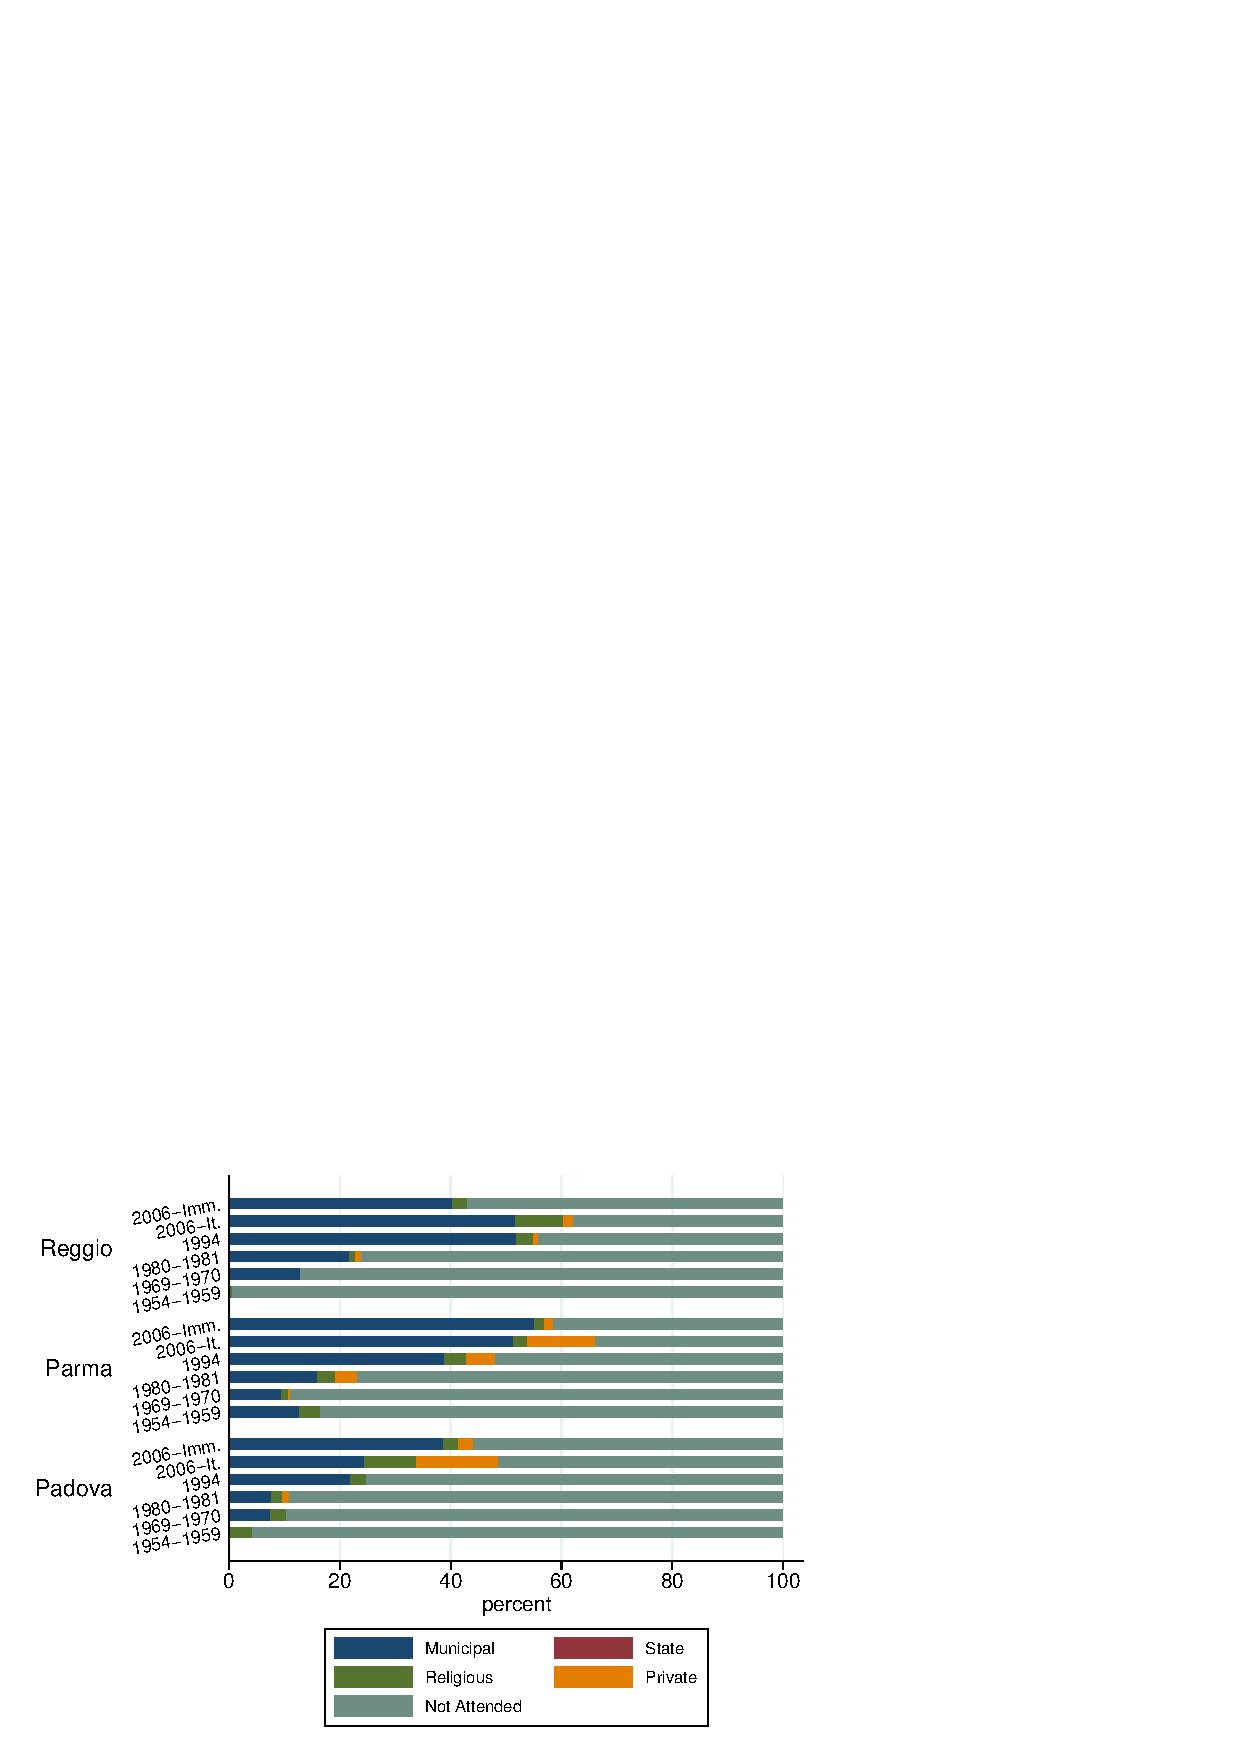
\includegraphics[height=8cm]{asiloType-Attend.png} \\[0pt]
\end{center}
\par
{\footnotesize {{\bfseries Notes:} Source: authors' calculations from the survey data. Type of infant-toddler center derived from parental section of the children and adolescent questionnaires providing type, name and address of childcare attended. Those who reported not to attend were either in other forms of childcare (e.g. nanny), or at home. It.=Italian. Imm.=Immigrant.} }
\end{figure}

\begin{figure}[!htb]
\caption{Type of Preschool attended, by city and cohort}
\label{fig:preschoolAttend}
\begin{center}
\includegraphics[height=8cm]{maternaType-Attend.png}\\[0pt]
\end{center}
\par
{\footnotesize {{\bfseries Notes:} Source: authors' calculations from the survey data. Type of preschool derived from parental section of the children and adolescent questionnaires providing type, name and address of childcare attended. Those who reported not to attend were either in other forms of childcare (e.g. nanny), or at home. It.=Italian. Imm.=Immigrant.} }
\end{figure}

As we can see from the data, the distribution of school type is quite different across cities and over the different cohorts. First of all, we can see that participation in preschool and, later on, also infant-toddler centers increased over time for all the three cities. Almost 40\% children and adolescents did not attend infant toddler centers while a negligible proportion have not attended preschool. For adults the situation is very different: the majority did not attend infant toddler centers, and a large proportion did not attend preschool either. Among the adults who have attended preschool, a large proportion attended religious schools. These strong differences among cohorts explain the need of a separate analysis between younger and older cohorts. Furthermore, when comparing across type of preschool, municipal infant-toddler centers and preschools are more popular in both Reggio Emilia and Parma, while religious centers are predominant in Padova. These differences remain quite constant overtime. \footnote{Again, note that these numbers are not necessarily representative of these cities and cohorts, but merely reflect our sample size, with an over sampling of municipal centers in the city of Reggio Emilia.} Private childcare centers entered the market later, and still represent a very small share of respondents.

\bigskip

Separate questionnaires were administered to the children, adolescents, and adults. as well as to the caregivers of the children and adolescents. The questionnaires include items about early childhood experiences, family structure, education, interaction with non-Italians (or with Italians in the case of the migrant children), and measures of cognitive and social-emotional skills. The questionnaires for adults additionally included items about occupation, income, health, and life satisfaction. 

Table \ref{table:summaryStat_baseline} presents summary statistics for baseline variables by cohort and city. As mentioned above, certain baseline variables are missing for the adult cohorts due to differences in questionnaires administered to adults and children. The table illustrates differences and similarities in parental, caregiver and family characteristics across cities as well as over time.

\begin{landscape}
\singlespace
\setlength{\tabcolsep}{2pt}
\begin{center}
\scriptsize{
\begin{longtable}{L{6cm} c c c p{.5cm} c c c p{.5cm} c c c p{.5cm} c c c p{.5cm} c c c}
\hline\multicolumn{20}{L{24cm}}{\textbf{Note:} Means are reported for each variable by cohort and city. Standard Deviations are reported in italics below each mean estimate. A . denotes that the variable is not defined for a specific cohort.}
\endfoot
\caption{Summary statistics for baseline variables by cohort and city} \label{table:summaryStat_baseline} \\
\hline
& \multicolumn{3}{c}{\textbf{Children}} & & \multicolumn{3}{c}{\textbf{Adolescents}} & & \multicolumn{3}{c}{\textbf{Adults 30}} & & \multicolumn{3}{c}{\textbf{Adults 40}} & & \multicolumn{3}{c}{\textbf{Adults 50}}\\
& \scriptsize{Reggio} & \scriptsize{Parma}& \scriptsize{Padova} & & \scriptsize{Reggio} & \scriptsize{Parma}& \scriptsize{Padova} & & \scriptsize{Reggio} & \scriptsize{Parma}& \scriptsize{Padova} & & \scriptsize{Reggio} & \scriptsize{Parma}& \scriptsize{Padova} & & \scriptsize{Reggio} & \scriptsize{Parma}& \scriptsize{Padova}\\
\hline \\[.2em] \endhead
 \quad Male & 0.54 &      0.56 &      0.52 & &      0.43 &      0.44 &      0.48 & &      0.60 &      0.53 &      0.55 & &      0.54 &      0.49 &      0.48 & &      0.47 &      0.38 &      0.46 \\*
 \quad & $\mathit{     0.50}$ & $\mathit{     0.50}$ & $\mathit{     0.50}$ & & $\mathit{     0.50}$ & $\mathit{     0.50}$ & $\mathit{     0.50}$ & & $\mathit{     0.49}$ & $\mathit{     0.50}$ & $\mathit{     0.50}$ & & $\mathit{     0.50}$ & $\mathit{     0.50}$ & $\mathit{     0.50}$ & & $\mathit{     0.50}$ & $\mathit{     0.49}$ & $\mathit{     0.50}$ \\[.2em]
 \quad Low birthweight & 0.08 &      0.07 &      0.05 & &      0.05 &      0.06 &      0.05 & &         . &         . &         . & &         . &         . &         . & &         . &         . &         . \\*
 \quad & $\mathit{     0.27}$ & $\mathit{     0.25}$ & $\mathit{     0.21}$ & & $\mathit{     0.23}$ & $\mathit{     0.24}$ & $\mathit{     0.21}$ & & $\mathit{        .}$ & $\mathit{        .}$ & $\mathit{        .}$ & & $\mathit{        .}$ & $\mathit{        .}$ & $\mathit{        .}$ & & $\mathit{        .}$ & $\mathit{        .}$ & $\mathit{        .}$ \\[.2em]
 \quad Premature birth & 0.10 &      0.08 &      0.07 & &      0.06 &      0.10 &      0.07 & &         . &         . &         . & &         . &         . &         . & &         . &         . &         . \\*
 \quad & $\mathit{     0.30}$ & $\mathit{     0.26}$ & $\mathit{     0.25}$ & & $\mathit{     0.24}$ & $\mathit{     0.30}$ & $\mathit{     0.25}$ & & $\mathit{        .}$ & $\mathit{        .}$ & $\mathit{        .}$ & & $\mathit{        .}$ & $\mathit{        .}$ & $\mathit{        .}$ & & $\mathit{        .}$ & $\mathit{        .}$ & $\mathit{        .}$ \\[.2em]
 \quad CAPI & 0.55 &      0.43 &      0.47 & &      0.43 &      0.55 &      0.49 & &      0.57 &      0.40 &      0.35 & &      0.63 &      0.34 &      0.35 & &      0.45 &      0.35 &      0.28 \\*
 \quad & $\mathit{     0.50}$ & $\mathit{     0.50}$ & $\mathit{     0.50}$ & & $\mathit{     0.50}$ & $\mathit{     0.50}$ & $\mathit{     0.50}$ & & $\mathit{     0.50}$ & $\mathit{     0.49}$ & $\mathit{     0.48}$ & & $\mathit{     0.48}$ & $\mathit{     0.48}$ & $\mathit{     0.48}$ & & $\mathit{     0.50}$ & $\mathit{     0.48}$ & $\mathit{     0.45}$ \\[.2em]
 \quad Born to teenaged mother & 0.00 &      0.01 &      0.01 & &      0.01 &      0.02 &      0.00 & &      1.00 &      1.00 &      1.00 & &      1.00 &      1.00 &      1.00 & &      1.00 &      1.00 &      1.00 \\*
 \quad & $\mathit{     0.00}$ & $\mathit{     0.08}$ & $\mathit{     0.08}$ & & $\mathit{     0.11}$ & $\mathit{     0.12}$ & $\mathit{     0.00}$ & & $\mathit{     0.00}$ & $\mathit{     0.00}$ & $\mathit{     0.00}$ & & $\mathit{     0.00}$ & $\mathit{     0.00}$ & $\mathit{     0.00}$ & & $\mathit{     0.00}$ & $\mathit{     0.00}$ & $\mathit{     0.00}$ \\[.2em]
 \quad Mom born in province & 0.51 &      0.60 &      0.69 & &      0.68 &      0.68 &      0.78 & &      0.84 &      0.70 &      0.71 & &      0.80 &      0.74 &      0.63 & &      0.78 &      0.80 &      0.76 \\*
 \quad & $\mathit{     0.50}$ & $\mathit{     0.49}$ & $\mathit{     0.46}$ & & $\mathit{     0.47}$ & $\mathit{     0.47}$ & $\mathit{     0.41}$ & & $\mathit{     0.36}$ & $\mathit{     0.46}$ & $\mathit{     0.46}$ & & $\mathit{     0.40}$ & $\mathit{     0.44}$ & $\mathit{     0.48}$ & & $\mathit{     0.42}$ & $\mathit{     0.40}$ & $\mathit{     0.43}$ \\[.2em]
 \quad Mom Max Edu: Low & 0.17 &      0.07 &      0.10 & &      0.16 &      0.11 &      0.14 & &      0.00 &      0.00 &      0.00 & &      0.02 &      0.00 &      0.00 & &      0.01 &      0.04 &      0.01 \\*
 \quad & $\mathit{     0.38}$ & $\mathit{     0.25}$ & $\mathit{     0.30}$ & & $\mathit{     0.36}$ & $\mathit{     0.31}$ & $\mathit{     0.35}$ & & $\mathit{     0.06}$ & $\mathit{     0.00}$ & $\mathit{     0.00}$ & & $\mathit{     0.13}$ & $\mathit{     0.00}$ & $\mathit{     0.06}$ & & $\mathit{     0.10}$ & $\mathit{     0.19}$ & $\mathit{     0.12}$ \\[.2em]
 \quad Mom Max Edu: Middle School & 0.08 &      0.05 &      0.09 & &      0.09 &      0.10 &      0.11 & &      0.03 &      0.07 &      0.10 & &      0.19 &      0.24 &      0.23 & &      0.41 &      0.55 &      0.64 \\*
 \quad & $\mathit{     0.27}$ & $\mathit{     0.23}$ & $\mathit{     0.29}$ & & $\mathit{     0.29}$ & $\mathit{     0.30}$ & $\mathit{     0.31}$ & & $\mathit{     0.18}$ & $\mathit{     0.25}$ & $\mathit{     0.30}$ & & $\mathit{     0.39}$ & $\mathit{     0.43}$ & $\mathit{     0.42}$ & & $\mathit{     0.49}$ & $\mathit{     0.50}$ & $\mathit{     0.48}$ \\[.2em]
 \quad Mom Max Edu: High School & 0.45 &      0.41 &      0.45 & &      0.48 &      0.44 &      0.43 & &      0.42 &      0.30 &      0.35 & &      0.47 &      0.35 &      0.35 & &      0.36 &      0.26 &      0.18 \\*
 \quad & $\mathit{     0.50}$ & $\mathit{     0.49}$ & $\mathit{     0.50}$ & & $\mathit{     0.50}$ & $\mathit{     0.50}$ & $\mathit{     0.50}$ & & $\mathit{     0.49}$ & $\mathit{     0.46}$ & $\mathit{     0.48}$ & & $\mathit{     0.50}$ & $\mathit{     0.48}$ & $\mathit{     0.48}$ & & $\mathit{     0.48}$ & $\mathit{     0.44}$ & $\mathit{     0.39}$ \\[.2em]
 \quad Mom Max Edu: University & 0.28 &      0.46 &      0.36 & &      0.25 &      0.33 &      0.29 & &      0.55 &      0.63 &      0.54 & &      0.31 &      0.41 &      0.41 & &      0.22 &      0.15 &      0.15 \\*
 \quad & $\mathit{     0.45}$ & $\mathit{     0.50}$ & $\mathit{     0.48}$ & & $\mathit{     0.43}$ & $\mathit{     0.47}$ & $\mathit{     0.46}$ & & $\mathit{     0.50}$ & $\mathit{     0.48}$ & $\mathit{     0.50}$ & & $\mathit{     0.46}$ & $\mathit{     0.49}$ & $\mathit{     0.49}$ & & $\mathit{     0.42}$ & $\mathit{     0.35}$ & $\mathit{     0.36}$ \\[.2em]
 \quad Born to teenaged father & 0.00 &      0.00 &      0.01 & &      0.00 &      0.01 &      0.00 & &      1.00 &      1.00 &      1.00 & &      1.00 &      1.00 &      1.00 & &      1.00 &      1.00 &      1.00 \\*
 \quad & $\mathit{     0.00}$ & $\mathit{     0.06}$ & $\mathit{     0.08}$ & & $\mathit{     0.00}$ & $\mathit{     0.09}$ & $\mathit{     0.06}$ & & $\mathit{     0.00}$ & $\mathit{     0.00}$ & $\mathit{     0.00}$ & & $\mathit{     0.00}$ & $\mathit{     0.00}$ & $\mathit{     0.00}$ & & $\mathit{     0.00}$ & $\mathit{     0.00}$ & $\mathit{     0.00}$ \\[.2em]
 \quad Father born in province & 0.52 &      0.59 &      0.64 & &      0.58 &      0.61 &      0.73 & &      0.87 &      0.79 &      0.76 & &      0.78 &      0.85 &      0.73 & &      0.84 &      0.65 &      0.82 \\*
 \quad & $\mathit{     0.50}$ & $\mathit{     0.49}$ & $\mathit{     0.48}$ & & $\mathit{     0.49}$ & $\mathit{     0.49}$ & $\mathit{     0.44}$ & & $\mathit{     0.34}$ & $\mathit{     0.41}$ & $\mathit{     0.43}$ & & $\mathit{     0.42}$ & $\mathit{     0.36}$ & $\mathit{     0.44}$ & & $\mathit{     0.37}$ & $\mathit{     0.48}$ & $\mathit{     0.38}$ \\[.2em]
 \quad Dad Max Edu: Low & 0.23 &      0.12 &      0.09 & &      0.19 &      0.16 &      0.14 & &         . &         . &         . & &      0.02 &      0.00 &      0.00 & &      0.01 &      0.04 &      0.02 \\*
 \quad & $\mathit{     0.42}$ & $\mathit{     0.33}$ & $\mathit{     0.29}$ & & $\mathit{     0.40}$ & $\mathit{     0.37}$ & $\mathit{     0.35}$ & & $\mathit{        .}$ & $\mathit{        .}$ & $\mathit{        .}$ & & $\mathit{     0.14}$ & $\mathit{     0.06}$ & $\mathit{     0.06}$ & & $\mathit{     0.07}$ & $\mathit{     0.19}$ & $\mathit{     0.14}$ \\[.2em]
 \quad Dad Max Edu: Middle School & 0.08 &      0.10 &      0.09 & &      0.09 &      0.07 &      0.10 & &      0.03 &      0.08 &      0.10 & &      0.19 &      0.22 &      0.14 & &      0.35 &      0.55 &      0.52 \\*
 \quad & $\mathit{     0.27}$ & $\mathit{     0.30}$ & $\mathit{     0.28}$ & & $\mathit{     0.28}$ & $\mathit{     0.26}$ & $\mathit{     0.30}$ & & $\mathit{     0.17}$ & $\mathit{     0.27}$ & $\mathit{     0.30}$ & & $\mathit{     0.39}$ & $\mathit{     0.41}$ & $\mathit{     0.35}$ & & $\mathit{     0.48}$ & $\mathit{     0.50}$ & $\mathit{     0.50}$ \\[.2em]
 \quad Dad Max Edu: High School & 0.35 &      0.36 &      0.42 & &      0.40 &      0.36 &      0.39 & &      0.37 &      0.32 &      0.32 & &      0.45 &      0.33 &      0.27 & &      0.36 &      0.19 &      0.17 \\*
 \quad & $\mathit{     0.48}$ & $\mathit{     0.48}$ & $\mathit{     0.49}$ & & $\mathit{     0.49}$ & $\mathit{     0.48}$ & $\mathit{     0.49}$ & & $\mathit{     0.48}$ & $\mathit{     0.47}$ & $\mathit{     0.47}$ & & $\mathit{     0.50}$ & $\mathit{     0.47}$ & $\mathit{     0.44}$ & & $\mathit{     0.48}$ & $\mathit{     0.40}$ & $\mathit{     0.38}$ \\[.2em]
 \quad Dad Max Edu: University & 0.24 &      0.35 &      0.30 & &      0.19 &      0.26 &      0.28 & &      0.60 &      0.60 &      0.57 & &      0.33 &      0.45 &      0.58 & &      0.27 &      0.20 &      0.27 \\*
 \quad & $\mathit{     0.43}$ & $\mathit{     0.48}$ & $\mathit{     0.46}$ & & $\mathit{     0.39}$ & $\mathit{     0.44}$ & $\mathit{     0.45}$ & & $\mathit{     0.49}$ & $\mathit{     0.49}$ & $\mathit{     0.50}$ & & $\mathit{     0.47}$ & $\mathit{     0.50}$ & $\mathit{     0.49}$ & & $\mathit{     0.45}$ & $\mathit{     0.40}$ & $\mathit{     0.45}$ \\[.2em]
 \quad Has 1 sibling & 0.52 &      0.46 &      0.50 & &      0.52 &      0.46 &      0.55 & &      0.36 &      0.33 &      0.45 & &      0.36 &      0.38 &      0.35 & &      0.28 &      0.26 &      0.39 \\*
 \quad & $\mathit{     0.50}$ & $\mathit{     0.50}$ & $\mathit{     0.50}$ & & $\mathit{     0.50}$ & $\mathit{     0.50}$ & $\mathit{     0.50}$ & & $\mathit{     0.48}$ & $\mathit{     0.47}$ & $\mathit{     0.50}$ & & $\mathit{     0.48}$ & $\mathit{     0.49}$ & $\mathit{     0.48}$ & & $\mathit{     0.45}$ & $\mathit{     0.44}$ & $\mathit{     0.49}$ \\[.2em]
 \quad Has 2 siblings & 0.14 &      0.21 &      0.17 & &      0.18 &      0.20 &      0.15 & &      0.24 &      0.33 &      0.25 & &      0.27 &      0.33 &      0.35 & &      0.30 &      0.27 &      0.22 \\*
 \quad & $\mathit{     0.35}$ & $\mathit{     0.41}$ & $\mathit{     0.37}$ & & $\mathit{     0.38}$ & $\mathit{     0.40}$ & $\mathit{     0.36}$ & & $\mathit{     0.43}$ & $\mathit{     0.47}$ & $\mathit{     0.43}$ & & $\mathit{     0.44}$ & $\mathit{     0.47}$ & $\mathit{     0.48}$ & & $\mathit{     0.46}$ & $\mathit{     0.45}$ & $\mathit{     0.42}$ \\[.2em]
 \quad Has more than 2 siblings & 0.06 &      0.04 &      0.05 & &      0.09 &      0.06 &      0.02 & &      0.13 &      0.20 &      0.17 & &      0.20 &      0.19 &      0.26 & &      0.34 &      0.39 &      0.35 \\*
 \quad & $\mathit{     0.23}$ & $\mathit{     0.19}$ & $\mathit{     0.21}$ & & $\mathit{     0.29}$ & $\mathit{     0.24}$ & $\mathit{     0.16}$ & & $\mathit{     0.33}$ & $\mathit{     0.40}$ & $\mathit{     0.37}$ & & $\mathit{     0.40}$ & $\mathit{     0.39}$ & $\mathit{     0.44}$ & & $\mathit{     0.48}$ & $\mathit{     0.49}$ & $\mathit{     0.48}$ \\[.2em]
 \quad Caregiver was Catholic & 0.77 &      0.83 &      0.79 & &      0.75 &      0.86 &      0.73 & &         . &         . &         . & &         . &         . &         . & &         . &         . &         . \\*
 \quad & $\mathit{     0.42}$ & $\mathit{     0.37}$ & $\mathit{     0.41}$ & & $\mathit{     0.43}$ & $\mathit{     0.35}$ & $\mathit{     0.44}$ & & $\mathit{        .}$ & $\mathit{        .}$ & $\mathit{        .}$ & & $\mathit{        .}$ & $\mathit{        .}$ & $\mathit{        .}$ & & $\mathit{        .}$ & $\mathit{        .}$ & $\mathit{        .}$ \\[.2em]
 \quad Caregiver was faithful and Catholic & 0.47 &      0.52 &      0.51 & &      0.45 &      0.54 &      0.45 & &         . &         . &         . & &         . &         . &         . & &         . &         . &         . \\*
 \quad & $\mathit{     0.50}$ & $\mathit{     0.50}$ & $\mathit{     0.50}$ & & $\mathit{     0.50}$ & $\mathit{     0.50}$ & $\mathit{     0.50}$ & & $\mathit{        .}$ & $\mathit{        .}$ & $\mathit{        .}$ & & $\mathit{        .}$ & $\mathit{        .}$ & $\mathit{        .}$ & & $\mathit{        .}$ & $\mathit{        .}$ & $\mathit{        .}$ \\[.2em]
 \quad Caregiver owned house & 0.58 &      0.71 &      0.66 & &      0.84 &      0.81 &      0.77 & &         . &         . &         . & &         . &         . &         . & &         . &         . &         . \\*
 \quad & $\mathit{     0.49}$ & $\mathit{     0.46}$ & $\mathit{     0.48}$ & & $\mathit{     0.37}$ & $\mathit{     0.39}$ & $\mathit{     0.42}$ & & $\mathit{        .}$ & $\mathit{        .}$ & $\mathit{        .}$ & & $\mathit{        .}$ & $\mathit{        .}$ & $\mathit{        .}$ & & $\mathit{        .}$ & $\mathit{        .}$ & $\mathit{        .}$ \\[.2em]
 \quad Caregiver was a migrant & 0.07 &      0.02 &      0.02 & &      0.01 &      0.02 &      0.00 & &         . &         . &         . & &         . &         . &         . & &         . &         . &         . \\*
 \quad & $\mathit{     0.26}$ & $\mathit{     0.14}$ & $\mathit{     0.15}$ & & $\mathit{     0.11}$ & $\mathit{     0.12}$ & $\mathit{     0.00}$ & & $\mathit{        .}$ & $\mathit{        .}$ & $\mathit{        .}$ & & $\mathit{        .}$ & $\mathit{        .}$ & $\mathit{        .}$ & & $\mathit{        .}$ & $\mathit{        .}$ & $\mathit{        .}$ \\[.2em]
 \quad Caregiver Income: 5,000 euros or less & 0.01 &      0.02 &      0.03 & &      0.00 &      0.02 &      0.04 & &         . &         . &         . & &         . &         . &         . & &         . &         . &         . \\*
 \quad & $\mathit{     0.11}$ & $\mathit{     0.15}$ & $\mathit{     0.18}$ & & $\mathit{     0.06}$ & $\mathit{     0.15}$ & $\mathit{     0.19}$ & & $\mathit{        .}$ & $\mathit{        .}$ & $\mathit{        .}$ & & $\mathit{        .}$ & $\mathit{        .}$ & $\mathit{        .}$ & & $\mathit{        .}$ & $\mathit{        .}$ & $\mathit{        .}$ \\[.2em]
 \quad Caregiver Income: 5,001-10,000 euros & 0.01 &      0.02 &      0.01 & &      0.01 &      0.01 &      0.01 & &         . &         . &         . & &         . &         . &         . & &         . &         . &         . \\*
 \quad & $\mathit{     0.11}$ & $\mathit{     0.13}$ & $\mathit{     0.12}$ & & $\mathit{     0.10}$ & $\mathit{     0.09}$ & $\mathit{     0.08}$ & & $\mathit{        .}$ & $\mathit{        .}$ & $\mathit{        .}$ & & $\mathit{        .}$ & $\mathit{        .}$ & $\mathit{        .}$ & & $\mathit{        .}$ & $\mathit{        .}$ & $\mathit{        .}$ \\[.2em]
 \quad Caregiver Income: 10,001-25,000 euros & 0.17 &      0.19 &      0.15 & &      0.18 &      0.18 &      0.10 & &         . &         . &         . & &         . &         . &         . & &         . &         . &         . \\*
 \quad & $\mathit{     0.38}$ & $\mathit{     0.39}$ & $\mathit{     0.36}$ & & $\mathit{     0.39}$ & $\mathit{     0.38}$ & $\mathit{     0.30}$ & & $\mathit{        .}$ & $\mathit{        .}$ & $\mathit{        .}$ & & $\mathit{        .}$ & $\mathit{        .}$ & $\mathit{        .}$ & & $\mathit{        .}$ & $\mathit{        .}$ & $\mathit{        .}$ \\[.2em]
 \quad Caregiver Income: 25,001-50,000 euros & 0.32 &      0.41 &      0.32 & &      0.32 &      0.29 &      0.24 & &         . &         . &         . & &         . &         . &         . & &         . &         . &         . \\*
 \quad & $\mathit{     0.47}$ & $\mathit{     0.49}$ & $\mathit{     0.47}$ & & $\mathit{     0.47}$ & $\mathit{     0.46}$ & $\mathit{     0.43}$ & & $\mathit{        .}$ & $\mathit{        .}$ & $\mathit{        .}$ & & $\mathit{        .}$ & $\mathit{        .}$ & $\mathit{        .}$ & & $\mathit{        .}$ & $\mathit{        .}$ & $\mathit{        .}$ \\[.2em]
 \quad Caregiver Income: 50,001-100,000 euros & 0.19 &      0.19 &      0.13 & &      0.24 &      0.24 &      0.11 & &         . &         . &         . & &         . &         . &         . & &         . &         . &         . \\*
 \quad & $\mathit{     0.40}$ & $\mathit{     0.39}$ & $\mathit{     0.34}$ & & $\mathit{     0.43}$ & $\mathit{     0.43}$ & $\mathit{     0.31}$ & & $\mathit{        .}$ & $\mathit{        .}$ & $\mathit{        .}$ & & $\mathit{        .}$ & $\mathit{        .}$ & $\mathit{        .}$ & & $\mathit{        .}$ & $\mathit{        .}$ & $\mathit{        .}$ \\[.2em]
 \quad Caregiver Income: 100,001-250,000 euros & 0.02 &      0.02 &      0.03 & &      0.04 &      0.03 &      0.02 & &         . &         . &         . & &         . &         . &         . & &         . &         . &         . \\*
 \quad & $\mathit{     0.15}$ & $\mathit{     0.14}$ & $\mathit{     0.17}$ & & $\mathit{     0.20}$ & $\mathit{     0.17}$ & $\mathit{     0.16}$ & & $\mathit{        .}$ & $\mathit{        .}$ & $\mathit{        .}$ & & $\mathit{        .}$ & $\mathit{        .}$ & $\mathit{        .}$ & & $\mathit{        .}$ & $\mathit{        .}$ & $\mathit{        .}$ \\[.2em]
 \quad Caregiver Income: > 250,000 euros & . &         . &         . & &      0.00 &      0.00 &      0.00 & &         . &         . &         . & &         . &         . &         . & &         . &         . &         . \\*
 \quad & $\mathit{        .}$ & $\mathit{        .}$ & $\mathit{        .}$ & & $\mathit{     0.06}$ & $\mathit{     0.00}$ & $\mathit{     0.00}$ & & $\mathit{        .}$ & $\mathit{        .}$ & $\mathit{        .}$ & & $\mathit{        .}$ & $\mathit{        .}$ & $\mathit{        .}$ & & $\mathit{        .}$ & $\mathit{        .}$ & $\mathit{        .}$ \\[.2em]
 \quad Caregiver was religious & 0.85 &      0.87 &      0.80 & &      0.77 &      0.87 &      0.74 & &      0.50 &      0.73 &      0.72 & &      0.50 &      0.75 &      0.75 & &      0.64 &      0.71 &      0.77 \\*
 \quad & $\mathit{     0.36}$ & $\mathit{     0.34}$ & $\mathit{     0.40}$ & & $\mathit{     0.42}$ & $\mathit{     0.34}$ & $\mathit{     0.44}$ & & $\mathit{     0.50}$ & $\mathit{     0.45}$ & $\mathit{     0.45}$ & & $\mathit{     0.50}$ & $\mathit{     0.43}$ & $\mathit{     0.44}$ & & $\mathit{     0.48}$ & $\mathit{     0.46}$ & $\mathit{     0.42}$ \\[.2em]
 ~\\[-.5em]
\hline
\end{longtable}
}
\end{center}

\end{landscape}


%%-------------------- Theoretical Approach ----------------------------------------------%
\section{Model of School Selection (Sketch)}
\label{sec:model}

In this section we sketch a theoretical framework which helps motivate and interpret our empirical results. In order to better understand the family decision to send the child to a Reggio Approach (RA) childcare center, consider a generalized Roy model framework. $Y_{1,i}$ represents the potential outcome of the child $i$ when attending an RA center, and $Y_{0,i}$ the potential outcome of the child when not attending an RA center. Define potential outcomes as follows:
\begin{align}
Y_{1,i}& =\beta_{1}(X_{i})+\varepsilon_{1,i} \nonumber \\
Y_{0,i}& =\beta_{0}(X_{i})+\varepsilon_{0,i} \nonumber \\
Y_{i} =& R_{i}Y_{1,i} + (1-R_{i}) Y_{1,i} \label{eq:outcome}
\end{align}%
where $\beta_{R}(X_{i})=E(Y_{R,i}|X=x)$ for $R=0,1$. The individual return to attending a Reggio Approach childcare center can be defined as the difference between these two potential outcomes, $\Delta_{i}^{RA}=Y_{1,i}-Y_{0,i}=\beta_{1}(X_{i})-\beta_{0}(X_{i})+\varepsilon_{1,i}-\varepsilon_{0,i}$.

The total costs of attending different types of preschools will systematically differ as well. First of all because public childcare is subsidized in Italy, and therefore the fees charged by municipal, state, and religious schools vary according to family income. %\todo[backgroundcolor=orange!30,size=\tiny]{Insert table about fees, either here or in the appendix}
Secondly, because each family might face a different disutility costs of sending a child to a particular type of school, depending on the family background or the distance to the different schools. 
Let the costs associated with attending or not an RA childcare center for family $i$ be given by:
\begin{equation*}
V_{R}(X_{i})=\gamma_{R}(X_{i})+\eta_{R,i},\ R=0,1,
\end{equation*}%
where $X_{i}$ are observable characteristics of household $i$, and $EV_{R}(X_{i})=\gamma_{R}(X_{i}).$

Finally, the probability of attending an RA center will joint depend on the supply and demand of childcare slots, that is on the family decision of demanding a spot $R_{d,i}=1$, and the likelihood of getting accepted $R_{s,i}=1$. 
A family will choose to demand a slot in a Reggio Approach center when facing a positive perceived net benefit, $R_{d,i}=1 \Leftrightarrow I_{R,i} \geq 0$:
\begin{eqnarray*}
I_{R_{d,i}} &=&\left(Y_{1,i}-V_{1,i}\right)-\left(Y_{0,i}-V_{0,i}\right) \geq 0 \\
%&=&\left(\beta_{1}(X_{i})-\beta_{0}(X_{i})+\varepsilon_{1,i}-\varepsilon_{0,i}\right)-\left(\gamma_{1}(X_{i})-\gamma_{0}(X_{i})+\eta_{1,i}-\eta_{0,i}\right) \\
&=&\beta_{1}(X_{i})-\beta_{0}(X_{i})-\gamma_{1}(X_{i})+\gamma_{0}(X_{i})-\omega_{d,i} \geq 0 
%\\ &=& h(X_{i}) \geq W_{i}
\end{eqnarray*}%
which is determined by the family observable characteristics $X_{i}$ and their unobservables $\omega_{d,i} \equiv \varepsilon_{0,i}-\varepsilon_{1,i}+\eta_{1,i}-\eta_{0,i}$. %and the net systematic return of demanding a slot in a RA center can be represented as $R_{d}(X_{i})=\beta_{d}(X_{i})-\gamma_{d}(X_{i})$. 
On the other hand, since the past decades have seen an excess of demand, priority access to public childcare slots was given according to very specific observable criteria $R_{s,i}=R_{s,i}(X_{i})$, which were publicly known and commonly decided in the city of Reggio Emilia.\footnote{See section (\ref{sec:ParmaPadova}) as well as \cite{Brilli2016} for more details}. %\todo[backgroundcolor=orange!30,size=\tiny]{More deatails about access}

Assuming linearity of the $\beta_{R}(\cdot)$ and $\gamma_{R}(\cdot)$ functions, the probability of household $i$ attending RA will depend on the following system of supply and demand equations:
%
\begin{align}
R_{s,i} = & \gamma_{s} \left(X_{i} \right) + \omega_{s,i}  \label{eq:1stage-supply} \\
R_{d,i} = & \gamma_{d} \left(X_{i} \right) + \omega_{d,i}  \label{eq:1stage-demand} 
%
%R_{s,i} = & \gamma_{x_{s}} X_{i} + \omega_{s,i}  \label{eq:1stage-supply} \\
%R_{d,i} = & \gamma_{x_{d}} X_{i} + \omega_{d,i}  \label{eq:1stage-demand} 
\end{align}
%
such that we will observe a child attending a RA center $R_{i}=1$ if and only if they apply $R_{d,i}=1$ and get accepted $R_{s,i}=1$.
%Note that the observables $Z_{s,i}$ and $Z_{d,i}$ are those characteristics of the household that shift the supply or the demand of childcare, but do not affect the potential academic and non-academic benefits of attending the two types of school. That is, the difference in attendance likelihoods for household $i$ are a function of the $X_{i}$ and $Z_{s,i}$ but the difference in school benefits between an RA school and a non-RA school are functions only of the observable characteristics $X_{i}$.

\bigskip

The variables observable to the econometrician are $R_{i},Y_{i}$ and $X_{i}$. Then we have the following system of equations:%
\begin{align}
E(R_{i}|X)        =&  \gamma \left(X_{i} \right) + \omega_{i}  \label{eq:1stage} \\
E(Y_{i} |X,R_{i})   =& R_{i} E(Y_{1,i}| R_{i}) + (1-R_{i}) E(Y_{0,i}| R_{i}) \nonumber \\
   %=& R_{i} E\left(\beta_{1}(X_{i})+\varepsilon_{1,i} | R_{i}\right) + (1-R_{i}) E \left(\beta_{0}(X_{i})+\varepsilon_{0,i} | R_{i}\right)  \nonumber \\
   %=& \beta_{0}(X_{i}) + R_{i} \left(\beta_{1}(X_{i}) - \beta_{0}(X_{i}) \right) + E(\varepsilon_{0,i}| R_{i})  + R_{i} E \left(\varepsilon_{1,i}  - \varepsilon_{0,i} | R_{i} \right) \nonumber \\
   =& \beta(X_{i}) + \delta R_{i} + E(\varepsilon_{R,i}| R_{i}) \label{eq:heckit}
\end{align}
where we have made the simplifying assumptions that $\beta_{1}(X_{i})=\beta_{0}(X_{i})=\beta(X_{i})$ up to differences in a constant $\delta$ which captures the average effect of attending an RA childcare center, and $\varepsilon_{R,i} \equiv \varepsilon_{0,i} +R_{i} (\varepsilon_{1,i}-\varepsilon_{0,i})$.
Now assume that all of the disturbance terms in the model are distributed as a multivariate normal. Then $\varepsilon_{R,i}, \omega_{i}$ are normally distributed, and the conditional expectation $E(\varepsilon_{R,i}|R_{i})$ in (\ref{eq:heckit}) can be consistently estimated (up to a scalar constant) from a first stage probit, as in \cite{Heckman1979}. We can then estimate the regression function with the estimated (up to scale) value $E(\varepsilon_{R,i}|R_{i}),$ and this enables identification of $\beta,\delta$ and a small set of elements of the covariance matrix of $W_{i}.$ More efficient estimates of the identified parameters can be obtained through joint estimation of the $R_{i}$ and $Y_{R,i}$ dependent variables.

%
%%--------------------   Empirical Approach ----------------------------------------------%

\section{Empirical Methods} \label{sec:method}

In order to evaluate the effect of Reggio Approach childcare centers on individual outcomes we adopt different econometric methodologies and different sub-samples of our data.

In term of methodology, we initially estimate the parameter $\hat{\delta}$ in equation (\ref{eq:heckit}) using Ordinary Least Squares; we then estimate the system of equations (\ref{eq:1stage}-\ref{eq:heckit}) using an Instrumental Variable approach, and two types of Propensity Score Matching; finally, we use a differences-in-differences strategy comparing Reggio Emilia with the other two control cities.

In terms of sub-samples, the data contains information on respondents from the city of Reggio Emilia, where some children were treated and some were not, and in the two control cities of Parma and Padova, where all children were untreated. The first sub-sample is composed of children in Reggio Emilia only. The identification strategy rests on the idea that, although all children could apply for a slot in the RA childcare, some were more likely to apply and obtain a slot due to some exogenous factors. The second sub-sample is composed of treated children in Reggio Emilia and all children in Parma and Padova. The underlying idea is that some children in Parma and Padova were very similar to treated children in Reggio Emilia, but were not treated simply because there were no RA centers in their city. The final two sub-sample leverage the differences between the two control cities of Parma and Padova, comparing children who attended municipal and non-municipal childcare in the cities of Reggio Emilia versus Parma, and children in Reggio Emilia versus Padova. The idea rests on the fact that, although parents may have had unobservable preferences to select a particular type of school instead of another, the effect of RA can be recovered under the assumption that the selection was similar across the different cities.

Here below we describe the ten specifications used to evaluate the impact of RA childcare centers, the results of which are reported in tables (\ref{tab:childIT}-\ref{tab:adoPS}) below. For each outcome $Y_{i}$ two parallel analysis are carried out: one estimating the effect of attending an RA infant-toddler center during ages 0-3, and another focusing on the effect of attending an RA preschool during ages 3-6.

\subsection{Reggio Emilia Only}

Focusing only on the respondents from Reggio Emilia, we first estimate with OLS the following linearisation of equation (\ref{eq:heckit}):
\begin{equation}
Y_{i} = \delta R_{i} + \alpha_{C} C_{i} + \beta X_{i} + \varepsilon_{i}    \hspace{2ex} \text{ if } i \in \text{Reggio Emilia} \label{eq1:OLSreggio}
\end{equation}

where $Y$ is the outcome of interest, the dummy variable $C_{i}$ indicates whether the child attended any type of childcare center, $R_{i}$ whether he attended a Reggio Approach infant-toddler center, and $X_{i}$ represents the vector of predetermined control variables (age and gender of the individual, health at birth, family structure, parental educational and economic resources, house property, religiosity, and distance from the town center).\footnote{For simplicity, we use `she' to refer to the mother, and `he' to refer to child, although we consider both genders in the regressions.} $\delta$ and $\alpha_{c}, \beta,$ are the parameters to be estimated, while only the parameter of interest $\hat{\delta}$ will be shown in the tables of results. If there is no systematic selection into RA centers, such that $E(\varepsilon|R=1)=E(\varepsilon|R=0)=E(\varepsilon)$, then OLS estimation of $\hat{\delta}$ in equation (\ref{eq1:OLSreggio}) measures the additional effect of attending a RA center rather than any other childcare center in Reggio Emilia.

%\medskip
%
%Worried about potential selection into RA given by the endogeneity of parental childcare decisions, we estimate the system of equations (\ref{eq:1stage}-\ref{eq:heckit}) instrumenting the RA dummy with variables $Z$ related to distance between the house and the closest RA childcare center, the score the child would have got if applying to an RA childcare center, mother's place of birth and whether she attended a childcare center when young:
%
%\begin{align}
%R_{i} =& \gamma_{z} Z_{i} + \gamma_{x} X_{i} + \omega_{i} \hspace{2ex} \text{ if } i \in \text{Reggio Emilia} \label{eq:est1stage} \\
%Y_{i} =& \delta \hat{R_{i}} + \alpha_{C} C_{i} + \beta X_{i} + \varepsilon_{i} \hspace{2ex} \text{ if } i \in \text{Reggio Emilia} \label{eq2:IVreggio}
%\end{align}
%
%\medskip
%
%As third specification, we adopt a control function strategy. We first estimate the probability to attend a RA infant-toddler center as in (\ref{eq:est1stage}) and then include in (\ref{eq1:OLSreggio}) a third degree polynomial of the difference between the actual RA choice and the RA predicted probability:%\footnote{We experimented with different degrees of polynomial without substantial differences in the results.}
%
%\begin{equation}
%Y_{i} = \delta \hat{R_{i}} + \alpha_{C} C_{i} + \beta X_{i} + \sum_p \theta_{p} \left(RA_{i} - \widehat{RA_{i}} \right)^{p} + \varepsilon_{i} \hspace{2ex} \text{ if } i \in \text{Reggio Emilia} \label{eq3:CFreggio}
%\end{equation}
%
%Results from (\ref{eq2:IVreggio}) and (\ref{eq3:CFreggio}) are valid under the assumption that the instruments are correlated with the RA choice but not with the outcome of interest.

\subsection{Treated in Reggio Emilia, control in Parma and Padova}

As additional specification, we again estimate using OLS equation (\ref{eq:heckit}), however this time we limit the sample to those children who attended an RA center, or those living in Parma or Padova, so that the parameter of interest is estimated as the additional effect of attending a RA infant-toddler in Reggio rather than any other infant-toddler center in Parma and Padova:
%
\begin{equation}
Y_{i} = \delta R_{i} + \alpha_{C} C_{i} + \beta X_{i} + \varepsilon_{i}    \hspace{2ex} \text{ if } i \in \{\text{RA } \cup \text{ Parma } \cup \text{ Padova } \} \label{eq4:OLSrpp}
\end{equation} 

\medskip

As another specification, in order to better approximate the observable characteristics of children in Parma and Padova who might have attended a RA center if only they were born in Reggio Emilia, we consider a Propensity Score Matching (PSM) approach. 
We apply to (\ref{eq4:OLSrpp}) probabilistic weights so that untreated children in Parma and Padova look similar -- considering weighted averages -- to treated children in Reggio Emilia. 
Probabilistic weights are calculated as:%
\begin{equation}
\left\{
\begin{tabular}{cl}
$\frac{1}{\widehat{R_{i}}}$   & if the child attended a RA school \\
$\frac{1}{1-\widehat{R_{i}}}$ & if the child did not attend a RA school
\end{tabular}
\right. \label{eq:weights}
\end{equation}
%
where the predicted probability of attending an RA center, $\widehat{R_{i}}$, is always obtained by equation (\ref{eq:est1stage}), estimated using only observations from Reggio Emilia.

%\medskip
%
%As a sixth specification, we take into consideration the fact that different observable characteristics drive the probability of demanding a slot in an RA center, and the probability of being accepted, as described in the system of equations (\ref{eq:1stage-supply}-\ref{eq:1stage-demand}).
%
%Probabilistic weights in this specification are calculated as:
%%
%\[
%\left\{
%\begin{tabular}{cl}
%$\frac{1}{ \widehat{R_{d,i}} \times \widehat{R_{s,i}}}$   & if the child attended a RA school \\
%$\frac{1}{1-\widehat{R_{d,i}}  \times \widehat{R_{s,i}}}$ & if the child did not attend a RA school
%\end{tabular}
%\right.
%\]
%%
%where $\widehat{R_{d,i}}$ is the estimated probability of demanding a RA childcare slot, and $\widehat{R_{s,i}}$ is the estimated probability of being offered a RA slot. These probabilites are estimated using a partial observability model in the spirit of \cite{Poirier1980}:
%
%\begin{align*}
%RA_{s,i} = & \gamma_{z_{s},IT} Z_{s,i} + \gamma_{x_{s},IT} X_{i} + \omega_{IT,s,i} \\
%RA_{d,i} = & \gamma_{z_{d},IT} Z_{d,i} + \gamma_{x_{d},IT} X_{i} + \omega_{IT,d,i} 
%\end{align*}
%
%where the instruments $Z$ are split according to their influence to the supply or demand function, and $\omega_{s,i}$ and $\omega_{s,i}$ are normally jointly distributed.

Results under th PSM specification are valid under the assumption that there are no other unobservable variables correlated with the RA choice and with the outcome of interest.

\subsection{Differences in Differences}

Finally, taking into consideration the fact that all cities have municipal schools but only in Reggio Emilia they follow the RA approach, we estimate the RA effect as the difference in outcomes between municipal and non-municipal schools in Reggio Emilia, compared to the difference in outcomes between municipal and non-municipal schools in Parma or Padova. The results using this differences-in-differences (DiD) approach are valid under the assumption that the selection into municipal centers is comparable in the three cities, and the difference in outcomes between municipal and non-municipal schools would have been the same in all the three cities in absence of the Reggio Approach.

First of all, we report as seventh specification the OLS estimate of usual linearisation of equation (\ref{eq:heckit}), this time only considering respondents in Reggio Emilia or Parma:
\begin{equation}
Y_{i} = \delta R_{i} + \alpha_{C} C_{i} + \beta X_{i} + \varepsilon_{i}    \hspace{2ex} \text{ if } i \in \text{Reggio Emilia } \cup \text{ Pr or Pd} \label{eq7:OLSrepr}
\end{equation}

\medskip

The DiD estimate in our eight specification is then achieved from the following equation, weighted using the same probabilistic weights estimated above in equation (\ref{eq:weights}):
\begin{align}
Y_{i} = \delta R_{i} + \alpha_{MC} MC_{i} + \alpha_{C} C_{i} + \alpha_{x} (C_{i} \times Reggio_{i}) &+  \alpha_{re} Reggio_{i} + \beta X_{i} + \varepsilon_{i} \nonumber \\
   & \text{ if } i \in \text{Reggio Emilia } \cup \text{ Parma} \label{eq8:didpr}
\end{align} 
%
where $Reggio_{i}=1$ if the respondent is from Reggio Emilia, $MC_{i}=1$ if the respondent attended a \textit{municipal} childcare center, and, just as before, $R_{i}=MC_{i} \times Reggio_{i}=1$ if the respondent attended a municipal childcare center in Reggio Emilia, therefore following the Reggio Approach.

\medskip

The last two specifications follow the same procedure, only that comparing Reggio Emilia with Padova:

\begin{align}
Y_{i} =& \delta R_{i} + \alpha_{C} C_{i} + \beta X_{i} + \varepsilon_{i}    \hspace{2ex} \text{ if } i \in \text{Reggio Emilia } \cup \text{ Padova} \label{eq9:OLSrepd} \\
Y_{i} =& \delta R_{i} + \alpha_{MC} MC_{i} + \alpha_{C} C_{i} + \alpha_{x} (C_{i} \times Reggio_{i}) +  \alpha_{re} Reggio_{i} + \beta X_{i} + \varepsilon_{i} \nonumber \\
& \hspace{25ex} \text{ if } i \in \text{Reggio Emilia } \cup \text{ Padova} \label{eq10:didpd}
\end{align}

%-------------------------------RESULTS------------------------%

\section{Results}
Given the differences in both outcome variables and control variables, we analyze the cohorts of children and adolescents separately from the adult ones.

\subsection{Children and Adolescents}
Following the estimation methods described above, we focus our attention on several outcomes $Y_{i}$ that capture various dimensions of the well being and human capital of these children and adolescents. Notably, we consider: measures of sociability (such as number of friends, whether the children would share candies with their best friend); measures of parental investment (having a musical instrument at home, reading to the child, whether the adolescents tells parents about activities done outside of the house, or about what happened at school); measures of socio-emotional skills (low scores on the Strength and Difficulties Questionnaire (SDQ), whether the child keeps his worries to himself, whether the child tells his worries to the teacher, high levels of trust); measures of health and healthy behaviors (BMI in normal ranges, self-reported good or excellent health, absence of any illness diagnosed by a physician, whether the child or adolescent eats fruit as a snack, whether the adolescent drinks or ever smoked); measures related to school (whether the child or adolescent had difficulties when starting elementary school such as lack of excitement, or difficulties in sitting still, whether the child or adolescent likes school, whether the adolescent is still in school); and finally measures of well-being (whether the child is happy in general, low adolescent scores on the CESD depression scale).

The summary statistics of these outcomes are reported in table (\ref{tab:childOutcomes}) for children and (\ref{tab:adoOutcomes}) for adolescents. To improve comparability, all $Y$ were converted into dummies equal to one in case of a favorable outcome,\footnote{For continous variables, the dummy was equal to 1 if the respondent was above the cohort-specific median.} such that a positive estimate of the coefficient $\hat{\delta}$ in any table represents a positive effect of participating to a RA childcare.

\begin{table}[ht]
\caption{Children Outcomes $Y$, age 6}
\label{tab:childOutcomes}
\begin{center}
    \begin{tabular}{lccc}
    \hline \hline
    City  & Reggio Emilia & Parma & Padova \\
    \hline

    Low SDQ score & 0.45  & 0.53** & 0.48 \\
          & [0.03] & [0.03] & [0.03] \\
    Talk about worries & 0.86  & 0.87  & 0.89 \\
          & [0.02] & [0.02] & [0.02] \\
    Tell worries to teacher & 0.3   & 0.3   & 0.21** \\
          & [0.03] & [0.03] & [0.02] \\
    Many friends & 0.43  & 0.37  & 0.48 \\
          & [0.03] & [0.03] & [0.03] \\
%    Happy in family & 0.71  & 0.58*** & 0.73 \\
%          & [0.03] & [0.03] & [0.03] \\
    Happy in general & 0.68  & 0.55*** & 0.71 \\
          & [0.03] & [0.03] & [0.03] \\
    Share candies & 0.89  & 0.94** & 0.94** \\
          & [0.02] & [0.01] & [0.01] \\
    Normal BMI & 0.77  & 0.84** & 0.85** \\
          & [0.03] & [0.02] & [0.02] \\
    Good health & 0.68  & 0.63  & 0.75* \\
          & [0.03] & [0.03] & [0.03] \\
    No illness & 0.75  & 0.78  & 0.83** \\
          & [0.02] & [0.02] & [0.02] \\
%    Never snacks & 0.95  & 0.95  & 0.94 \\
%          & [0.01] & [0.01] & [0.01] \\
    Fruit as snack & 0.44  & 0.47  & 0.5 \\
          & [0.03] & [0.03] & [0.03] \\
    Musical instr. at home & 0.47  & 0.46  & 0.54* \\
          & [0.03] & [0.03] & [0.03] \\
    Often read to child & 0.56  & 0.73*** & 0.56 \\
          & [0.03] & [0.03] & [0.03] \\
%    Art or drama class & 0.05  & 0.06  & 0.06 \\
%          & [0.01] & [0.02] & [0.01] \\
%    Music or dance class & 0.17  & 0.17  & 0.22 \\
%          & [0.02] & [0.02] & [0.03] \\
    Excited to learn & 0.97  & 0.95  & 0.95 \\
          & [0.01] & [0.01] & [0.01] \\
    Can sit still & 0.86  & 0.86  & 0.9 \\
          & [0.02] & [0.02] & [0.02] \\
    Likes school & 0.66  & 0.73* & 0.52*** \\
          & [0.03] & [0.03] & [0.03] \\


    \hline	
    \end{tabular}
\end{center}

\begin{footnotesize}
\raggedright{Share of respondents reporting a positive outcome across the three cities. Standard errors in brackets.
Non-parametric test of differences in means between Reggio Emilia and the other city shown as *** $p<0.01$, ** $p<0.05$, * $p<0.1$.}
\end{footnotesize}
\end{table}

\begin{table}[ht]
\caption{Adolescents Outcomes $Y$, age 18}
\label{tab:adoOutcomes}
\begin{center}
    \begin{tabular}{lccc}
    \hline \hline
    City  & Reggio Emilia & Parma & Padova \\
    \hline

    Low SDQ score & 0.52  & 0.54  & 0.48 \\
          & [0.03] & [0.03] & [0.03] \\
    Talks about activities & 0.56  & 0.41*** & 0.57 \\
          & [0.03] & [0.03] & [0.03] \\
    Talks about school & 0.62  & 0.48*** & 0.65 \\
          & [0.03] & [0.03] & [0.03] \\
%    Close to dad & 0.39  & 0.4   & 0.39 \\
%          & [0.03] & [0.03] & [0.03] \\
%    Close to mom & 0.56  & 0.51  & 0.46** \\
%          & [0.03] & [0.03] & [0.03] \\
    Many friends & 0.54  & 0.49  & 0.59 \\
          & [0.03] & [0.03] & [0.03] \\
%    Satisfied & 0.59  & 0.47*** & 0.62 \\
%          & [0.03] & [0.03] & [0.03] \\
    Low depression score & 0.46  & 0.47  & 0.57** \\
          & [0.03] & [0.03] & [0.03] \\
    High trust & 0.51  & 0.60* & 0.53 \\
          & [0.03] & [0.03] & [0.03] \\
    Normal BMI & 0.66  & 0.69  & 0.62 \\
          & [0.03] & [0.03] & [0.03] \\
    Good health & 0.67  & 0.53*** & 0.7 \\
          & [0.03] & [0.03] & [0.03] \\
    No illness & 0.66  & 0.65  & 0.75** \\
          & [0.03] & [0.03] & [0.03] \\
%    Never snacks & 0.87  & 0.79** & 0.84 \\
%          & [0.02] & [0.03] & [0.02] \\
    Fruit as snack & 0.37  & 0.25*** & 0.35 \\
          & [0.03] & [0.03] & [0.03] \\
    Never smoked & 0.55  & 0.44** & 0.56 \\
          & [0.03] & [0.03] & [0.03] \\
    Doesn't drink & 0.46  & 0.39  & 0.52 \\
          & [0.03] & [0.03] & [0.03] \\
    Excited to learn & 0.96  & 0.97  & 0.96 \\
          & [0.01] & [0.01] & [0.01] \\
    Can sit still & 0.94  & 0.89* & 0.91 \\
          & [0.01] & [0.02] & [0.02] \\
    Attending school & 0.96  & 0.97  & 0.99** \\
          & [0.01] & [0.01] & [0.01] \\
    Likes school & 0.72  & 0.68  & 0.69 \\
          & [0.03] & [0.03] & [0.03] \\

    \hline	
    \end{tabular}
\end{center}

\begin{footnotesize}
\raggedright{Share of adolescents reporting a positive outcome across the three cities. Standard errors in brackets.
Non-parametric test of differences in means between Reggio Emilia and the other city shown as *** $p<0.01$, ** $p<0.05$, * $p<0.1$.}
\end{footnotesize}
\end{table}

Turning now to the estimation results, tables (\ref{tab:childIT}) reports the effect of attending an RA infant-toddler center and (\ref{tab:childPS}) the effect of attending an RA preschool estimated according to the methods describe in the previous section, and focusing on the sample of children aged 6. Tables (\ref{tab:adoIT}) and (\ref{tab:adoPS}) instead focus on the sample of adolescents aged 18.
The reported coefficients have large confidence intervals, and few estimates are always significant across all the different methods and samples considered. This represents a strength of this approach, since it allows us to focus only on the results that are strong and consistent regardless of the particular identification approach chosen.

Overall we find evidence of positive effects in the social domain, especially pertaining to number of friends and relationships with the parents, and more favorable outcomes in school, especially in term of fewer difficulties when starting elementary school. Although both children and adolescents report better healthy behaviors, such as eating fruit, the differences in terms of health are not always positive or significant. Finally, we do discover some negative effects: the caregivers of children report investing slightly less at home, and adolescents display a lower lever of trust. Here below we consider all of these results in greater detail, first for children and then for adolescents.

\subsection{Children}
For children aged 6, table (\ref{tab:childIT}) shows that participation to an RA infant-toddler center is consistently related to a higher number of friends, fewer difficulties entering elementary school, but also a higher body-mass-index, as reported by the caregiver. 
With respect to health measures, there are no significant differences in health benefits, neither in terms of fewer number of diagnosis (although faring better when compared to Parma or Padova separately, children attending RA do not report fewer diagnosis than other children in Reggio Emilia), or in terms of self-reported health; even if RA children are more likely to report eating fruit as a snack, such differences are not statistically significant.
With respect to socio-emotional measures, children attending an RA infant-toddler center are more likely to confide to a teacher when feeling worries, but reports from child-reported happiness, and from the Strengths and Difficulties Questionnaire (SDQ) are seldom significant and move from positive to negative depending on the specification.
Finally, in term of investments, no clear picture arises.

As shown in table (\ref{tab:childPS}), children attending a RA preschool seem to be better adapted to elementary school: they are more likely to go to a teacher when they are worried, are less likely to have difficulties in being excited to learn, or sitting still, and generally report liking school more.
With respect to health measures, they do not fare better in terms of Body-Mass-Index, and report better health only when compared to similar children in Parma. 
Regarding socio-emotional skills, self-reported happiness and mother-reports from the SDQ are often positive but not consistently so.
Finally, caregivers seem to invest slightly less if they send their children to an RA preschool, notably they are less likely to read often to the child.


%-------------------------------------------------------see childAsilo.tex
\begin{table}[ht]
\caption{Estimated effect of attending an RA infant-toddler center, children age 6}

\label{tab:childIT}
\begin{center}
\begin{adjustbox}{width=1.2\textwidth,center=\textwidth}
\small
%begin{tabular}{m{2.0cm} cccc}
\begin{tabular}{lccccccc}
\hline 
 & {(1) } & {(2) } & {(3) } & {(4) } & {(5) } & {(6) } & {(7) }\\
{Method } & {OLS } & {OLS } & {PSM } & {OLS } & {DiD Pr } & {OLS } & {DiD Pd }\\
{Sample } & {Reggio } & {RA-Pr-Pd } & {RA-Pr-Pd } & {Re-Pr } & {Re-Pr } & {Re-Pd } & {Re-Pd }\\
\hline 
{Low SDQ score } & {0.139 } & {-0.003 } & {-0.021 } & {0.046 } & {0.008 } & {0.118{*} } & {0.165 }\\
 & [0.089] & [0.049] & [0.058] & [0.069] & [0.168] & [0.069] & [0.167]\\
{Talk about worries } & {-0.034 } & {0.018 } & {0.001 } & {0.009 } & {-0.055 } & {0.014 } & {-0.086 }\\
 & [0.057] & [0.035] & [0.035] & [0.045] & [0.078] & [0.046] & [0.084]\\
{Tell worries to teacher } & {-0.010 } & {0.074 } & {0.090{*} } & {-0.009 } & {-0.067 } & {0.078 } & {-0.184 }\\
 & [0.093] & [0.047] & [0.053] & [0.066] & [0.140] & [0.064] & [0.138]\\
{Many friends } & {0.104 } & {-0.028 } & {0.011 } & {0.132{*} } & {0.280{*}{*} } & {0.031 } & {0.394{*}{*}{*} }\\
 & [0.090] & [0.048] & [0.055] & [0.068] & [0.141] & [0.069] & [0.127]\\
{%Happy in family & -0.033 & -0.435 & -0.020 & 0.027 & 0.033 & 0.524*** & -0.084 & -0.032 & -0.076 & -0.119 \\% & [0.092] & [0.602] & [0.211] & [0.047] & [0.053] & [0.170] & [0.067] & [0.133] & [0.064] & [0.130] \\Happy
in general } & {0.034 } & {0.042 } & {0.028 } & {-0.018 } & {0.008 } & {0.004 } & {0.075 }\\
 & [0.097] & [0.047] & [0.053] & [0.069] & [0.138] & [0.067] & [0.135]\\
{Share candies } & {0.025 } & {-0.024 } & {-0.019 } & {0.023 } & {0.149{*} } & {0.029 } & {-0.041 }\\
 & [0.043] & [0.027] & [0.027] & [0.039] & [0.081] & [0.037] & [0.063]\\
{Normal BMI } & {-0.139{*} } & {-0.085{*}{*} } & {-0.123{*}{*}{*} } & {-0.072 } & {-0.180 } & {-0.067 } & {-0.142 }\\
 & [0.078] & [0.042] & [0.045] & [0.060] & [0.110] & [0.059] & [0.087]\\
{Good health } & {-0.027 } & {-0.040 } & {-0.023 } & {-0.026 } & {-0.110 } & {-0.088 } & {0.042 }\\
 & [0.087] & [0.046] & [0.055] & [0.067] & [0.172] & [0.064] & [0.133]\\
{No illness } & {0.133 } & {-0.081{*} } & {-0.041 } & {-0.077 } & {0.253{*} } & {-0.011 } & {0.328{*}{*} }\\
 & [0.097] & [0.043] & [0.048] & [0.067] & [0.151] & [0.063] & [0.135]\\
{%Never snacks & 0.027 & 0.242 & 0.012 & -0.006 & 0.011 & 0.033 & -0.024 & 0.032 & 0.021 & 0.055 \\% & [0.053] & [0.440] & [0.115] & [0.023] & [0.028] & [0.042] & [0.035] & [0.066] & [0.034] & [0.082] \\Fruit
as snack } & {0.107 } & {-0.065 } & {-0.019 } & {-0.011 } & {0.077 } & {-0.017 } & {0.150 }\\
 & [0.100] & [0.049] & [0.057] & [0.072] & [0.181] & [0.072] & [0.165]\\
{Musical instr. at home } & {-0.014 } & {0.006 } & {0.015 } & {0.119{*} } & {0.115 } & {-0.046 } & {-0.243{*} }\\
 & [0.097] & [0.050] & [0.058] & [0.070] & [0.140] & [0.069] & [0.130]\\
{Often read to child } & {0.006 } & {-0.052 } & {-0.120{*}{*} } & {0.093 } & {-0.260{*} } & {-0.044 } & {-0.035 }\\
 & [0.095] & [0.045] & [0.050] & [0.066] & [0.134] & [0.068] & [0.124]\\
{%Art or drama class  & -0.155** & -0.485* & -0.199** & -0.021 & -0.014 & 0.071 & -0.067 & -0.085 & -0.050 & -0.182* \\% & [0.075] & [0.275] & [0.096] & [0.022] & [0.024] & [0.086] & [0.044] & [0.134] & [0.042] & [0.101] \\%Music or dance class  & -0.019 & 0.142 & 0.064 & 0.017 & -0.014 & 0.104 & 0.032 & -0.006 & 0.003 & -0.042 \\% & [0.080] & [0.457] & [0.174] & [0.040] & [0.045] & [0.097] & [0.057] & [0.092] & [0.057] & [0.105] \\Excited
to learn } & {0.017 } & {0.030{*} } & {0.030{*} } & {0.014 } & {0.065{*} } & {0.023 } & {0.053 }\\
 & [0.036] & [0.016] & [0.017] & [0.026] & [0.037] & [0.026] & [0.050]\\
{Can sit still } & {-0.042 } & {0.021 } & {0.035 } & {0.006 } & {0.119 } & {0.094{*}{*} } & {0.116 }\\
 & [0.051] & [0.032] & [0.033] & [0.047] & [0.078] & [0.046] & [0.092]\\
{Likes school } & {0.018 } & {0.090{*}{*} } & {0.037 } & {0.080 } & {-0.307{*}{*} } & {0.127{*} } & {0.066 }\\
 & [0.095] & [0.045] & [0.051] & [0.065] & [0.137] & [0.068] & [0.140]\\
\hline 
{N obs. } & {309 } & {725 } & {722 } & {597 } & {593 } & {586 } & {583 }\\
\hline 
\end{tabular}
\end{adjustbox}
\end{center}

\begin{footnotesize}
\raggedright{Robust standard errors in brackets. *** $p<0.01$, ** $p<0.05$, * $p<0.1$. Sample: Reggio = only respondents in the city of Reggio Emilia. RA-Pr-Pd = Reggio Approach and all the respondents in Parma and Padova. Re-Pr= all of the respondents in Reggio Emilia and Parma. Re-Pd= all of the respondents in Reggio Emilia and Padova. Estimation method: OLS = Ordinary Least Square; PSM = simple propensity score matching. DiD = differences-in-differences approach municipal schools vs other schools across different cities}
\end{footnotesize}
\end{table}


%-------------------------------------------------------see childMaterna.tex
\begin{table}[ht]
\caption{Estimated effect of attending an RA preschool, children age 6}
\label{tab:childPS}
\begin{center}
\begin{adjustbox}{width=1.2\textwidth,center=\textwidth}
\small
%begin{tabular}{m{2.0cm} cccc}
\begin{tabular}{lccccccc}
\hline 
 & {(1) } & {(2) } & {(3) } & {(4) } & {(5) } & {(6) } & {(7) }\\
{Method } & {OLS } & {OLS } & {PSM } & {OLS } & {DiD Pr } & {OLS } & {DiD Pd }\\
{Sample } & {Reggio } & {RA-Pr-Pd } & {RA-Pr-Pd } & {Re-Pr } & {Re-Pr } & {Re-Pd } & {Re-Pd }\\
\hline 
{Low SDQ score } & {0.089 } & {0.005 } & {-0.049 } & {0.093 } & {-0.284{*}{*} } & {0.084 } & {0.218{*}{*} }\\
 & [0.057] & [0.046] & [0.058] & [0.056] & [0.117] & [0.056] & [0.091]\\
{Talk about worries } & {0.050 } & {0.021 } & {-0.081 } & {0.058 } & {-0.080 } & {0.047 } & {-0.185{*} }\\
 & [0.040] & [0.029] & [0.062] & [0.040] & [0.074] & [0.040] & [0.100]\\
{Tell worries to teacher } & {0.080 } & {0.084{*} } & {0.106{*} } & {0.057 } & {0.609{*}{*}{*} } & {0.084 } & {0.031 }\\
 & [0.053] & [0.043] & [0.061] & [0.053] & [0.109] & [0.052] & [0.091]\\
{Many friends } & {-0.058 } & {-0.092{*}{*} } & {-0.053 } & {-0.063 } & {-0.309{*}{*}{*} } & {-0.054 } & {0.338{*}{*} }\\
 & [0.057] & [0.044] & [0.076] & [0.056] & [0.081] & [0.056] & [0.150]\\
{%Happy in family & -0.046 & 0.091 & -0.010 & 0.029 & -0.004 & 0.036 & -0.057 & 0.160** & -0.048 & -0.300** \\% & [0.054] & [0.212] & [0.228] & [0.043] & [0.060] & [0.078] & [0.052] & [0.080] & [0.052] & [0.137] \\Happy
in general } & {0.035 } & {0.037 } & {0.010 } & {0.036 } & {0.243{*}{*}{*} } & {0.023 } & {-0.070 }\\
 & [0.057] & [0.043] & [0.067] & [0.055] & [0.084] & [0.055] & [0.180]\\
{Share candies } & {0.032 } & {-0.029 } & {-0.098 } & {0.029 } & {0.329{*}{*} } & {0.024 } & {-0.136 }\\
 & [0.037] & [0.025] & [0.062] & [0.036] & [0.144] & [0.036] & [0.089]\\
{Normal BMI } & {-0.022 } & {-0.055 } & {-0.080 } & {0.001 } & {0.172{*}{*} } & {0.005 } & {-0.071 }\\
 & [0.055] & [0.041] & [0.052] & [0.053] & [0.079] & [0.053] & [0.074]\\
{Good health } & {0.007 } & {-0.024 } & {0.051 } & {-0.013 } & {0.411{*}{*}{*} } & {-0.017 } & {-0.088 }\\
 & [0.054] & [0.041] & [0.061] & [0.053] & [0.121] & [0.053] & [0.069]\\
{No illness } & {0.046 } & {-0.015 } & {0.094{*} } & {0.040 } & {0.147 } & {0.045 } & {0.200{*} }\\
 & [0.053] & [0.038] & [0.056] & [0.051] & [0.089] & [0.051] & [0.107]\\
{%Never snacks & 0.032 & -0.083 & -0.041 & 0.017 & 0.053 & -0.030 & 0.038 & -0.376*** & 0.032 & 0.150 \\% & [0.027] & [0.132] & [0.136] & [0.019] & [0.048] & [0.047] & [0.026] & [0.081] & [0.026] & [0.127] \\Fruit
as snack } & {0.041 } & {-0.024 } & {-0.033 } & {0.036 } & {-0.096 } & {0.036 } & {0.165{*} }\\
 & [0.058] & [0.046] & [0.054] & [0.057] & [0.094] & [0.057] & [0.095]\\
{Musical instr. at home } & {0.001 } & {-0.024 } & {0.015 } & {-0.012 } & {-0.028 } & {-0.002 } & {0.080 }\\
 & [0.057] & [0.044] & [0.065] & [0.057] & [0.115] & [0.057] & [0.085]\\
{Often read to child } & {-0.052 } & {-0.082{*} } & {-0.135{*}{*} } & {-0.049 } & {-0.185{*}{*} } & {-0.060 } & {-0.087 }\\
 & [0.056] & [0.044] & [0.061] & [0.055] & [0.085] & [0.055] & [0.091]\\
{%Art or drama class  & -0.049* & -0.037 & -0.017 & -0.038** & -0.024 & -0.016 & -0.058** & 0.060 & -0.054* & -0.042 \\% & [0.027] & [0.057] & [0.073] & [0.018] & [0.029] & [0.031] & [0.028] & [0.062] & [0.028] & [0.040] \\%Music or dance class  & -0.090* & -0.283 & -0.316 & -0.040 & -0.096* & -0.006 & -0.090* & -0.195** & -0.088* & -0.056 \\% & [0.047] & [0.211] & [0.242] & [0.033] & [0.050] & [0.038] & [0.046] & [0.092] & [0.047] & [0.068] \\Excited
to learn } & {0.011 } & {0.026 } & {0.071{*}{*} } & {0.014 } & {-0.062 } & {0.015 } & {0.368{*}{*}{*} }\\
 & [0.021] & [0.016] & [0.031] & [0.020] & [0.052] & [0.020] & [0.114]\\
{Can sit still } & {-0.002 } & {-0.017 } & {-0.025 } & {-0.002 } & {0.196{*}{*}{*} } & {-0.001 } & {0.143{*} }\\
 & [0.040] & [0.030] & [0.046] & [0.040] & [0.063] & [0.039] & [0.076]\\
{Likes school } & {0.076 } & {0.067 } & {0.109{*} } & {0.070 } & {0.449{*}{*}{*} } & {0.084 } & {0.443{*}{*}{*} }\\
 & [0.056] & [0.042] & [0.063] & [0.054] & [0.118] & [0.054] & [0.112]\\
\hline 
{N obs. } & {305 } & {711 } & {708 } & {590 } & {587 } & {565 } & {563 }\\
\hline 
\end{tabular}
\end{adjustbox}
\end{center}

\begin{footnotesize}
\raggedright{Robust standard errors in brackets. *** $p<0.01$, ** $p<0.05$, * $p<0.1$. Sample: Reggio = only respondents in the city of Reggio Emilia. RA-Pr-Pd = Reggio Approach and all the respondents in Parma and Padova. Re-Pr= all of the respondents in Reggio Emilia and Parma. Re-Pd= all of the respondents in Reggio Emilia and Padova. Estimation method: OLS = Ordinary Least Square; PSM = simple propensity score matching. DiD = differences-in-differences approach municipal schools vs other schools across different cities}
\end{footnotesize}
\end{table}

\subsection{Adolescents}
Let's now focus on the estimated effects of attending RA centers for adolescents.

The most consistent result in table (\ref{tab:adoIT}) is that adolescents who attended an RA infant-toddler center report having many more friends. They also seem to have a better relationship with their parents: they are more likely to talk with them about events happening at school or outside of the house. However, their mental health is not improved: they are marginally more likely to be depressed, and less likely to reporting a high level of trust.
In terms of health, they do not appear slimmer in terms of BMI, however their reported health seems better, and they do not seem to suffer from more diagnosed diseases. They do report healthier behaviours: they are more likely to choose a fruit as a snack; although no significant differences in drinking appear, they are less likely to report ever smoking (with the exception of when compared to adolescents in Padova). 
In terms of schooling, they are less likely to be a high-school dropout, are marginally less likely to have had difficulties when starting elementary school, but they do not report liking school more.

The estimated effect of attending an RA preschool are reported in table (\ref{tab:adoPS}), where we find slightly fewer consistently significant results. Notably, their reported health is always higher than comparable adolescents who did not attend RA preschools, and they are more likely to report healthy behaviours such as eating fruit and never having smoked. 
Regarding the relationships with their parents, they seem to be slightly more likely to talk with them about events happening outside the house. 
In terms of schooling, they are also less likely to report being a dropout, and marginal but not significant positive results can be found also when considering difficulties when entering elementary school, or how much they like school. 
Finally, their mental health doesn't seem to be different from other adolescents: their estimated effect on the depression score is positive but never significant, while the probability of reporting a high level of trust is marginally negative.


%-------------------------------------------------------see adoAsilo.tex
\begin{table}[ht]
\caption{Estimated effect of attending an RA infant-toddler center, adolescents age 18}

\label{tab:adoIT}
\begin{center}
\begin{adjustbox}{width=1.2\textwidth,center=\textwidth}
\small
%begin{tabular}{m{2.0cm} cccc}
\begin{tabular}{lccccccc}
\hline 
 & {(1) } & {(2) } & {(3) } & {(4) } & {(5) } & {(6) } & {(7) }\\
{Method } & {OLS } & {OLS } & {PSM } & {OLS } & {DiD Pr } & {OLS } & {DiD Pd }\\
{Sample } & {Reggio } & {RA-Pr-Pd } & {RA-Pr-Pd } & {Re-Pr } & {Re-Pr } & {Re-Pd } & {Re-Pd }\\
\hline 
{Low SDQ score } & {-0.026 } & {0.059 } & {-0.068 } & {0.148{*} } & {-0.349 } & {0.024 } & {0.192 }\\
 & [0.160] & [0.055] & [0.073] & [0.081] & [0.259] & [0.084] & [0.264]\\
{Talks about activities } & {-0.057 } & {0.190{*}{*}{*} } & {0.294{*}{*}{*} } & {0.088 } & {-0.049 } & {0.072 } & {-0.192 }\\
 & [0.152] & [0.054] & [0.070] & [0.079] & [0.189] & [0.083] & [0.266]\\
{Talks about school } & {0.052 } & {0.174{*}{*}{*} } & {0.294{*}{*}{*} } & {0.090 } & {0.340{*} } & {0.124 } & {-0.242 }\\
 & [0.156] & [0.052] & [0.068] & [0.078] & [0.198] & [0.080] & [0.283]\\
{%Close to dad & 0.109 & -1.775 & 0.295 & 0.051 & 0.064 & 0.018 & 0.134* & 0.240 & 0.067 & 0.475* \\% & [0.144] & [1.440] & [0.270] & [0.054] & [0.070] & [0.057] & [0.077] & [0.204] & [0.082] & [0.285] \\%Close to mom & 0.039 & -0.797 & -0.030 & 0.163*** & 0.026 & 0.120** & 0.117 & 0.120 & 0.186** & 0.500 \\% & [0.153] & [1.112] & [0.282] & [0.054] & [0.071] & [0.057] & [0.080] & [0.243] & [0.081] & [0.306] \\Many
friends } & {0.422{*}{*}{*} } & {0.126{*}{*} } & {0.208{*}{*}{*} } & {0.231{*}{*}{*} } & {0.485{*} } & {0.178{*}{*} } & {0.095 }\\
 & [0.139] & [0.054] & [0.073] & [0.078] & [0.258] & [0.081] & [0.288]\\
{%Satisfied & 0.043 & 1.245 & 0.109 & 0.146*** & 0.187** & 0.142** & 0.068 & 0.340 & 0.129 & 0.461* \\% & [0.150] & [1.150] & [0.294] & [0.056] & [0.074] & [0.058] & [0.081] & [0.241] & [0.083] & [0.251] \\Low
depression score } & {-0.249{*} } & {-0.005 } & {-0.003 } & {-0.068 } & {-0.123 } & {0.018 } & {-0.462{*} }\\
 & [0.144] & [0.056] & [0.079] & [0.080] & [0.212] & [0.084] & [0.253]\\
{High trust } & {-0.216 } & {-0.135{*}{*} } & {-0.139{*} } & {-0.080 } & {-0.064 } & {-0.177{*}{*} } & {-0.285 }\\
 & [0.154] & [0.055] & [0.079] & [0.081] & [0.232] & [0.084] & [0.334]\\
{Normal BMI } & {-0.145 } & {-0.018 } & {-0.045 } & {0.026 } & {0.160 } & {-0.002 } & {0.252 }\\
 & [0.107] & [0.051] & [0.068] & [0.074] & [0.199] & [0.073] & [0.213]\\
{Good health } & {-0.139 } & {0.197{*}{*}{*} } & {0.151{*} } & {0.099 } & {-0.044 } & {0.088 } & {0.019 }\\
 & [0.108] & [0.054] & [0.082] & [0.077] & [0.191] & [0.077] & [0.232]\\
{No illness } & {-0.036 } & {0.038 } & {0.101 } & {0.082 } & {-0.317 } & {0.038 } & {0.470{*}{*} }\\
 & [0.144] & [0.053] & [0.067] & [0.077] & [0.220] & [0.077] & [0.187]\\
{%Never snacks & 0.066 & 1.340 & 0.079 & 0.091** & 0.296*** & 0.089** & 0.091 & 0.334*** & 0.066 & 0.100 \\% & [0.122] & [0.847] & [0.220] & [0.040] & [0.067] & [0.040] & [0.060] & [0.125] & [0.059] & [0.241] \\Fruit
as snack } & {0.188 } & {0.157{*}{*}{*} } & {0.266{*}{*}{*} } & {0.152{*}{*} } & {0.154 } & {0.171{*}{*} } & {-0.030 }\\
 & [0.126] & [0.053] & [0.057] & [0.074] & [0.174] & [0.079] & [0.205]\\
{Never smoked } & {0.292{*}{*} } & {0.091{*} } & {0.092 } & {0.064 } & {0.138 } & {0.053 } & {-0.465{*}{*} }\\
 & [0.136] & [0.055] & [0.072] & [0.080] & [0.211] & [0.084] & [0.196]\\
{Does not drink } & {-0.162 } & {0.079 } & {0.104 } & {-0.031 } & {-0.256 } & {0.051 } & {-0.263 }\\
 & [0.162] & [0.055] & [0.079] & [0.081] & [0.203] & [0.084] & [0.276]\\
{Excited to learn } & {-0.022 } & {0.010 } & {0.014 } & {0.025 } & {-0.009 } & {0.015 } & {0.216{*}{*} }\\
 & [0.024] & [0.019] & [0.023] & [0.026] & [0.023] & [0.030] & [0.102]\\
{Can sit still } & {-0.023 } & {0.050{*} } & {0.013 } & {0.016 } & {-0.105 } & {0.020 } & {0.029 }\\
 & [0.027] & [0.030] & [0.034] & [0.041] & [0.091] & [0.040] & [0.136]\\
{Attending school } & {0.005 } & {0.029 } & {0.022{*} } & {0.089{*}{*}{*} } & {0.010 } & {0.050{*}{*} } & {0.016 }\\
 & [0.027] & [0.019] & [0.013] & [0.029] & [0.046] & [0.024] & [0.024]\\
{Likes school } & {0.147 } & {0.064 } & {0.000 } & {0.061 } & {-0.100 } & {0.053 } & {0.085 }\\
 & [0.130] & [0.051] & [0.058] & [0.074] & [0.197] & [0.077] & [0.276]\\
\hline 
{N obs. } & {291 } & {669 } & {631 } & {536 } & {503 } & {564 } & {531 }\\
\hline 
\end{tabular}
\end{adjustbox}
\end{center}

\begin{footnotesize}
\raggedright{Robust standard errors in brackets. *** $p<0.01$, ** $p<0.05$, * $p<0.1$. Sample: Reggio = only respondents in the city of Reggio Emilia. RA-Pr-Pd = Reggio Approach and all the respondents in Parma and Padova. Re-Pr= all of the respondents in Reggio Emilia and Parma. Re-Pd= all of the respondents in Reggio Emilia and Padova. Estimation method: OLS = Ordinary Least Square; PSM = simple propensity score matching. DiD = differences-in-differences approach municipal schools vs other schools across different cities}
\end{footnotesize}
\end{table}

%-------------------------------------------------------see adoMaterna.tex
\begin{table}[ht]
\caption{Estimated effect of attending an RA preschool, adolescents age 18}
\label{tab:adoPS}
\begin{center}
\begin{adjustbox}{width=1.2\textwidth,center=\textwidth}
\small
%begin{tabular}{m{2.0cm} cccc}
\begin{tabular}{lccccccc}
\hline 
 & {(1) } & {(2) } & {(3) } & {(4) } & {(5) } & {(6) } & {(7) }\\
{Method } & {OLS } & {OLS } & {PSM } & {OLS } & {DiD Pr } & {OLS } & {DiD Pd }\\
{Sample } & {Reggio } & {RA-Pr-Pd } & {RA-Pr-Pd } & {Re-Pr } & {Re-Pr } & {Re-Pd } & {Re-Pd }\\
\hline 
{Low SDQ score } & {0.014 } & {0.035 } & {0.026 } & {0.037 } & {0.035 } & {0.031 } & {0.008 }\\
 & [0.062] & [0.047] & [0.049] & [0.061] & [0.095] & [0.060] & [0.099]\\
{Talks about activities } & {-0.009 } & {0.089{*} } & {0.082{*} } & {-0.015 } & {-0.046 } & {-0.008 } & {0.017 }\\
 & [0.062] & [0.046] & [0.048] & [0.060] & [0.093] & [0.059] & [0.098]\\
{Talks about school } & {-0.023 } & {0.058 } & {0.052 } & {-0.017 } & {-0.068 } & {-0.019 } & {-0.096 }\\
 & [0.059] & [0.045] & [0.048] & [0.059] & [0.091] & [0.058] & [0.087]\\
{%Close to dad & 0.036 & 0.114 & -0.228 & 0.018 & 0.010 & 0.015 & 0.038 & 0.095 & 0.031 & 0.021 \\% & [0.060] & [0.300] & [0.429] & [0.046] & [0.048] & [0.046] & [0.059] & [0.086] & [0.059] & [0.099] \\%Close to mom & -0.110* & 0.034 & -0.017 & 0.018 & 0.008 & 0.017 & -0.110* & -0.120 & -0.093 & -0.149 \\% & [0.061] & [0.319] & [0.439] & [0.046] & [0.048] & [0.046] & [0.060] & [0.095] & [0.059] & [0.099] \\Many
friends } & {0.060 } & {0.053 } & {0.048 } & {0.046 } & {0.047 } & {0.061 } & {0.047 }\\
 & [0.059] & [0.045] & [0.048] & [0.059] & [0.095] & [0.058] & [0.097]\\
{%Satisfied & -0.033 & -0.129 & -0.542 & 0.051 & 0.046 & 0.053 & -0.039 & -0.128 & -0.030 & -0.091 \\% & [0.060] & [0.294] & [0.380] & [0.046] & [0.048] & [0.047] & [0.059] & [0.091] & [0.060] & [0.093] \\Low
depression score } & {0.059 } & {0.022 } & {0.014 } & {0.078 } & {0.041 } & {0.065 } & {0.079 }\\
 & [0.062] & [0.047] & [0.049] & [0.061] & [0.093] & [0.060] & [0.095]\\
{High trust } & {-0.045 } & {-0.090{*} } & {-0.065 } & {-0.050 } & {-0.041 } & {-0.044 } & {0.040 }\\
 & [0.062] & [0.047] & [0.049] & [0.060] & [0.094] & [0.061] & [0.099]\\
{Normal BMI } & {0.034 } & {-0.041 } & {-0.036 } & {0.015 } & {0.158{*} } & {0.025 } & {-0.046 }\\
 & [0.058] & [0.043] & [0.045] & [0.057] & [0.087] & [0.056] & [0.089]\\
{Good health } & {0.087 } & {0.131{*}{*}{*} } & {0.134{*}{*}{*} } & {0.066 } & {0.150{*} } & {0.068 } & {0.093 }\\
 & [0.058] & [0.044] & [0.046] & [0.057] & [0.091] & [0.057] & [0.089]\\
{No illness } & {-0.045 } & {-0.040 } & {-0.045 } & {-0.036 } & {-0.037 } & {-0.042 } & {-0.002 }\\
 & [0.059] & [0.044] & [0.046] & [0.057] & [0.092] & [0.057] & [0.086]\\
{%Never snacks & 0.026 & 0.047 & 0.057 & 0.039 & 0.029 & 0.040 & 0.016 & -0.006 & 0.028 & -0.005 \\% & [0.045] & [0.163] & [0.228] & [0.033] & [0.035] & [0.033] & [0.044] & [0.070] & [0.043] & [0.064] \\Fruit
as snack } & {0.158{*}{*}{*} } & {0.139{*}{*}{*} } & {0.145{*}{*}{*} } & {0.158{*}{*}{*} } & {0.238{*}{*}{*} } & {0.167{*}{*}{*} } & {0.154 }\\
 & [0.057] & [0.046] & [0.047] & [0.057] & [0.077] & [0.056] & [0.095]\\
{Never smoked } & {0.039 } & {0.086{*} } & {0.082{*} } & {0.055 } & {0.068 } & {0.048 } & {-0.083 }\\
 & [0.062] & [0.046] & [0.047] & [0.060] & [0.094] & [0.060] & [0.097]\\
{Does not drink } & {-0.023 } & {0.026 } & {0.022 } & {-0.011 } & {0.054 } & {-0.025 } & {-0.098 }\\
 & [0.061] & [0.047] & [0.048] & [0.061] & [0.094] & [0.060] & [0.097]\\
{Excited to learn } & {0.034 } & {0.009 } & {0.004 } & {0.029 } & {0.084{*}{*} } & {0.034 } & {0.021 }\\
 & [0.025] & [0.015] & [0.016] & [0.025] & [0.036] & [0.025] & [0.039]\\
{Can sit still } & {0.004 } & {0.038 } & {0.042 } & {0.006 } & {0.038 } & {0.006 } & {0.043 }\\
 & [0.029] & [0.024] & [0.025] & [0.029] & [0.061] & [0.029] & [0.061]\\
{Attending school } & {0.055{*}{*} } & {-0.000 } & {0.000 } & {0.051{*}{*} } & {0.094{*}{*} } & {0.048{*} } & {0.063{*} }\\
 & [0.027] & [0.015] & [0.017] & [0.026] & [0.041] & [0.026] & [0.034]\\
{Likes school } & {0.032 } & {0.055 } & {0.077{*} } & {0.051 } & {0.065 } & {0.052 } & {0.045 }\\
 & [0.057] & [0.043] & [0.042] & [0.055] & [0.088] & [0.055] & [0.093]\\
\hline 
{N obs. } & {291 } & {678 } & {644 } & {536 } & {534 } & {564 } & {531 }\\
\hline 
\end{tabular}
\end{adjustbox}
\end{center}

\begin{footnotesize}
\raggedright{Robust standard errors in brackets. *** $p<0.01$, ** $p<0.05$, * $p<0.1$. Sample: Reggio = only respondents in the city of Reggio Emilia. RA-Pr-Pd = Reggio Approach and all the respondents in Parma and Padova. Re-Pr= all of the respondents in Reggio Emilia and Parma. Re-Pd= all of the respondents in Reggio Emilia and Padova. Estimation method: OLS = Ordinary Least Square; PSM = simple propensity score matching. DiD = differences-in-differences approach municipal schools vs other schools across different cities}
\end{footnotesize}
\end{table}

\subsection{Adults}
We now turn to the analysis of adult outcomes for the different cohorts. We again follow a similar identification strategy; however, given the more limited amount of information regarding the background family characteristics of adults, we consider two different sets of possible control variables $X$. First we report the results without any control, therefore displaying a difference in means; secondly, we consider a limited set of controls that were chosen in order to minimize the Bayesian Information Criterion (BIC); finally, we consider a full set of controls including dummies for mother and father education, socio-economic status, and level of religiosity.

Furthermore, given the very limited number of individuals who attended an Infant-toddler-center (ages 0-3), we focus our analysis on participation in preschool.

Tables \ref{ols-E-reg} to \ref{ols-S-reg} show OLS estimate on the participation of the Reggio Approach preschools for people in Reggio who attended Reggio Approach preschools or no preschool at all. We do not include the age-50 cohort in this analysis, as the Reggio Approach did not exist for that cohort. We perform analysis using (i) no control, (ii) 6 controls selected by Bayesian Information Criterion (BIC), and (iii) the full set of controls that include baseline variables available for the adult cohorts. 


Table \ref{ols-W-reg} shows consistently significant positive effects of the Reggio Approach on hours worked per week. Moreover, there are significant effects on the indicator for the lowest household income category for the age-40 cohort. Note that the measures for subject labor income, including ``Monthly Wage'' presented in the table, have very few observations. Household income suffers less from the missing value problem.

Table \ref{ols-L-reg} shows significant effects of the Reggio Approach on the status of being divorced for the age-30 cohort. Other results do not show any significant trend. 

Table \ref{ols-H-reg} show that the significantly increasing effects of the Reggio Approach on numbers of days sick for the past month at the time of the interview for the age-30 cohort. Moreover, the results show the significant decreasing effects on whether the respondent has ever been suspended from school. 

Table \ref{ols-N-reg} shows no consistently significant trends between the age-30 cohort and age-40 cohort. For the age-30 cohort, there are significantly decreasing effects on the optimistic look in life. Moreover, there are significantly increasing effects on whether the respondent is likely to do the same to someone who puts him/her in a difficult situation and to someone who insults him/her.
For the age-40 cohort, results show the significantly decreasing effects on depression for the age-30 cohort. There are also significantly positive effects on satisfaction with income and with work for the age-40 cohort. However, there are significantly positive effects on whether the respondent thinks work is source of stress. 

Finally, table \ref{ols-S-reg} shows consistently significant and negative effects of the Reggio Approach on whether the respondent does volunteer work for both the age-30 and age-40 cohorts. Moreover, for the age-40 cohort, there are significantly negative effects on respondents having migrant friends and significantly positive effects on whether respondents have ever voted for municipal and regional elections. For the age-30 cohort, there are significantly negative effects on whether respondents have ever voted for national elections.




% ========================================================================= %
% ADULT COHORT

\begin{landscape}
\singlespacing
%\subsection{Preschool (Ages 3-6), Adult Cohorts}

\begin{table}[H] \caption{OLS and Diff-in-Diff for Cognitive and Education, Preschools, Adult Cohorts} \label{ols-E-reg}
\scalebox{0.80}{{
\def\sym#1{\ifmmode^{#1}\else\(^{#1}\)\fi}
\begin{tabular}{l*{10}{c}}
\toprule
            &\multicolumn{1}{c}{(1)}&\multicolumn{1}{c}{(2)}&\multicolumn{1}{c}{(3)}&\multicolumn{1}{c}{(4)}&\multicolumn{1}{c}{(5)}&\multicolumn{1}{c}{(6)}&\multicolumn{1}{c}{(7)}&\multicolumn{1}{c}{(8)}&\multicolumn{1}{c}{(9)}&\multicolumn{1}{c}{(10)}\\
            &\multicolumn{1}{c}{None30}&\multicolumn{1}{c}{BIC30}&\multicolumn{1}{c}{Full30}&\multicolumn{1}{c}{DidPm30}&\multicolumn{1}{c}{DidPv30}&\multicolumn{1}{c}{None40}&\multicolumn{1}{c}{BIC40}&\multicolumn{1}{c}{Full40}&\multicolumn{1}{c}{DidPm40}&\multicolumn{1}{c}{DidPv40}\\
\midrule
IQ Factor   &     -0.0740         &      -0.225         &      -0.204         &      -0.438\sym{**} &     -0.0628         &     -0.0745         &     -0.0492         &     -0.0363         &       0.269         &       0.402         \\
            &     (0.139)         &     (0.122)         &     (0.127)         &     (0.157)         &     (0.218)         &     (0.109)         &     (0.110)         &     (0.113)         &     (0.232)         &     (0.247)         \\
\addlinespace
High School Grade&       3.803\sym{**} &       4.697\sym{**} &       4.564\sym{**} &       3.230         &       3.868         &     0.00175         &       0.451         &       0.579         &      -0.485         &       1.298         \\
            &     (1.446)         &     (1.537)         &     (1.547)         &     (3.348)         &     (3.597)         &     (1.311)         &     (1.320)         &     (1.417)         &     (5.488)         &     (3.121)         \\
\addlinespace
University Grade&       2.577         &       2.606         &       2.344         &       4.426         &       1.200         &      -1.818         &      -1.763         &      -3.197         &      -1.431         &      -4.171         \\
            &     (1.851)         &     (2.021)         &     (2.035)         &     (3.292)         &     (3.469)         &     (2.196)         &     (2.196)         &     (2.931)         &     (3.032)         &     (3.505)         \\
\addlinespace
Graduate from High School&     -0.0328         &    -0.00368         &     -0.0135         &       0.169\sym{*}  &     -0.0848         &      0.0233         &      0.0442         &      0.0573         &      -0.120         &     -0.0718         \\
            &    (0.0441)         &    (0.0410)         &    (0.0430)         &    (0.0757)         &    (0.0693)         &    (0.0495)         &    (0.0489)         &    (0.0545)         &    (0.0768)         &    (0.0874)         \\
\addlinespace
Max Edu: University&    -0.00935         &      0.0300         &      0.0212         &       0.195\sym{*}  &       0.137         &      0.0432         &      0.0543         &      0.0585         &      -0.262         &      0.0133         \\
            &    (0.0585)         &    (0.0578)         &    (0.0598)         &    (0.0926)         &     (0.133)         &    (0.0505)         &    (0.0492)         &    (0.0466)         &     (0.158)         &     (0.126)         \\
\addlinespace
Max Edu: Graduate School&           0         &           0         &           0         &      0.0166         &       0.102\sym{***}&           0         &           0         &           0         &     -0.0711         &     -0.0249         \\
            &         (.)         &         (.)         &         (.)         &    (0.0102)         &    (0.0253)         &         (.)         &         (.)         &         (.)         &    (0.0939)         &    (0.0525)         \\
\bottomrule
\end{tabular}
}
}
\vspace{1ex} \\
\footnotesize\raggedright{Note: This table shows the estimates of the coefficient for attending Reggio Approach preschools from the OLS and difference-in-difference (DiD) models. Column title indicates the corresponding age group, control set, and model. ``None30'' refers to the OLS estimate with only the age-30 cohort and with no control variables. ``BIC30'' refers to the OLS estimate with only the age-30 cohort and with controls selected by Bayesian Information Criterion (BIC). ``Full30'' refers to the OLS estimate with only the age-30 cohort and with the full set of controls. ``DidPm30'' refers to the difference-in-difference estimate of (Reggio Muni - Parma Muni) - (Reggio None - Parma None) for the age-30 cohort. ``DidPv30'' refers to the difference-in-difference estimate of (Reggio Muni - Padova Muni) - (Reggio None - Padova None) for the age-30 cohort.  Analogous meanings are applied to the age-40 cohort in columns (7) through (12). Robust standard errors are reported in parentheses. Stars show statistical significance as follows: * $p < 0.05$, ** $p < 0.01$, *** $p < 0.001$.}
\end{table}

\begin{table}[H] \caption{OLS and Diff-in-Diff for Employment and Income, Preschools, Adult Cohorts} \label{ols-W-reg}
\scalebox{0.76}{
{
\def\sym#1{\ifmmode^{#1}\else\(^{#1}\)\fi}
\begin{tabular}{l*{10}{c}}
\toprule
            &\multicolumn{1}{c}{(1)}&\multicolumn{1}{c}{(2)}&\multicolumn{1}{c}{(3)}&\multicolumn{1}{c}{(4)}&\multicolumn{1}{c}{(5)}&\multicolumn{1}{c}{(6)}&\multicolumn{1}{c}{(7)}&\multicolumn{1}{c}{(8)}&\multicolumn{1}{c}{(9)}&\multicolumn{1}{c}{(10)}\\
            &\multicolumn{1}{c}{None30}&\multicolumn{1}{c}{BIC30}&\multicolumn{1}{c}{Full30}&\multicolumn{1}{c}{DidPm30}&\multicolumn{1}{c}{DidPv30}&\multicolumn{1}{c}{None40}&\multicolumn{1}{c}{BIC40}&\multicolumn{1}{c}{Full40}&\multicolumn{1}{c}{DidPm40}&\multicolumn{1}{c}{DidPv40}\\
\midrule
Employed    &      0.0158         &    0.000343         &      0.0214         &      0.0322         &     -0.0111         &      0.0333         &      0.0313         &      0.0195         &    -0.00602         &     -0.0885\sym{*}  \\
            &    (0.0332)         &    (0.0325)         &    (0.0321)         &    (0.0673)         &    (0.0864)         &    (0.0279)         &    (0.0249)         &    (0.0271)         &    (0.0357)         &    (0.0396)         \\
\addlinespace
Self-Employed&     -0.0466         &     -0.0616         &     -0.0591         &     -0.0980         &      0.0302         &     -0.0451         &     -0.0529         &     -0.0555         &      -0.127         &      0.0684         \\
            &    (0.0462)         &    (0.0451)         &    (0.0471)         &    (0.0709)         &    (0.0512)         &    (0.0456)         &    (0.0461)         &    (0.0477)         &     (0.133)         &    (0.0534)         \\
\addlinespace
Hours Worked Per Week&       4.252\sym{***}&       3.388\sym{**} &       2.793\sym{*}  &       3.110         &       4.067\sym{*}  &       1.281         &       1.270         &       1.391         &       1.557         &       3.019         \\
            &     (1.177)         &     (1.139)         &     (1.106)         &     (2.079)         &     (1.666)         &     (1.405)         &     (1.416)         &     (1.472)         &     (2.465)         &     (3.121)         \\
\addlinespace
Monthly Wage&      -21.31         &      -91.92         &       16.74         &      -113.0         &       62.54         &      -135.4         &      -153.4         &      -202.5         &           0         &       405.1         \\
            &     (90.62)         &     (93.95)         &     (87.36)         &     (221.4)         &     (208.5)         &     (588.3)         &     (538.6)         &     (566.1)         &         (.)         &     (859.3)         \\
\addlinespace
Income: 5,000 Euros of Less&      0.0420         &      0.0500         &      0.0372         &      0.0521         &    -0.00310         &     -0.0132         &     -0.0149         &     -0.0164         &    -0.00710         &     -0.0128         \\
            &    (0.0346)         &    (0.0344)         &    (0.0313)         &    (0.0334)         &    (0.0664)         &   (0.00934)         &    (0.0106)         &    (0.0119)         &    (0.0158)         &   (0.00942)         \\
\addlinespace
Income: 5,001-10,000 Euros&    -0.00660         &    0.000813         &     0.00386         &      0.0147         &      0.0106         &    -0.00662         &     -0.0111         &    -0.00756         &    -0.00316         &     0.00758         \\
            &    (0.0161)         &    (0.0174)         &    (0.0142)         &    (0.0187)         &    (0.0191)         &   (0.00663)         &    (0.0109)         &   (0.00766)         &    (0.0104)         &    (0.0164)         \\
\addlinespace
Income: 10,001-25,000 Euros&      -0.113         &      -0.103         &      -0.108         &     -0.0256         &     -0.0709         &     -0.0779         &     -0.0701         &     -0.0763         &       0.259\sym{***}&      -0.232         \\
            &    (0.0644)         &    (0.0652)         &    (0.0691)         &     (0.113)         &     (0.135)         &    (0.0586)         &    (0.0584)         &    (0.0622)         &    (0.0715)         &     (0.139)         \\
\addlinespace
Income: 25,001-50,000 Euros&      0.0400         &      0.0266         &      0.0387         &      0.0409         &      0.0109         &       0.101         &       0.105         &      0.0826         &      -0.118         &       0.180         \\
            &    (0.0692)         &    (0.0703)         &    (0.0716)         &     (0.116)         &     (0.136)         &    (0.0650)         &    (0.0656)         &    (0.0701)         &     (0.152)         &     (0.143)         \\
\addlinespace
Income: 50,001-100,000 Euros&      0.0380         &      0.0255         &      0.0287         &     -0.0909         &      0.0486         &      0.0227         &     0.00965         &      0.0250         &      -0.115         &      0.0685         \\
            &    (0.0293)         &    (0.0275)         &    (0.0287)         &    (0.0697)         &    (0.0617)         &    (0.0363)         &    (0.0387)         &    (0.0399)         &     (0.131)         &    (0.0732)         \\
\addlinespace
Income: 100,001-250,000 Euros&           0         &           0         &           0         &     0.00883         &     0.00394         &     -0.0263         &     -0.0186         &    -0.00735         &     -0.0153         &     -0.0116         \\
            &         (.)         &         (.)         &         (.)         &   (0.00889)         &   (0.00420)         &    (0.0271)         &    (0.0284)         &    (0.0300)         &    (0.0282)         &    (0.0282)         \\
\addlinespace
Income: More than 250,000 Euros&           0         &           0         &           0         &           0         &           0         &           0         &           0         &           0         &           0         &           0         \\
            &         (.)         &         (.)         &         (.)         &         (.)         &         (.)         &         (.)         &         (.)         &         (.)         &         (.)         &         (.)         \\
\bottomrule
\end{tabular}
}
}
\vspace{1ex} \\
\footnotesize\raggedright{Note: This table shows the estimates of the coefficient for attending Reggio Approach preschools from the OLS and difference-in-difference (DiD) models. Column title indicates the corresponding age group, control set, and model. ``None30'' refers to the OLS estimate with only the age-30 cohort and with no control variables. ``BIC30'' refers to the OLS estimate with only the age-30 cohort and with controls selected by Bayesian Information Criterion (BIC). ``Full30'' refers to the OLS estimate with only the age-30 cohort and with the full set of controls. ``DidPm30'' refers to the difference-in-difference estimate of (Reggio Muni - Parma Muni) - (Reggio None - Parma None) for the age-30 cohort. ``DidPv30'' refers to the difference-in-difference estimate of (Reggio Muni - Padova Muni) - (Reggio None - Padova None) for the age-30 cohort.  Analogous meanings are applied to the age-40 cohort in columns (7) through (12). Robust standard errors are reported in parentheses. Stars show statistical significance as follows: * $p < 0.05$, ** $p < 0.01$, *** $p < 0.001$.}
\end{table}

\begin{table}[H] \caption{OLS and Diff-in-Diff for Living Environment, Preschools, Adult Cohorts} \label{ols-L-reg}
\scalebox{0.80}{
{
\def\sym#1{\ifmmode^{#1}\else\(^{#1}\)\fi}
\begin{tabular}{l*{10}{c}}
\toprule
            &\multicolumn{1}{c}{(1)}&\multicolumn{1}{c}{(2)}&\multicolumn{1}{c}{(3)}&\multicolumn{1}{c}{(4)}&\multicolumn{1}{c}{(5)}&\multicolumn{1}{c}{(6)}&\multicolumn{1}{c}{(7)}&\multicolumn{1}{c}{(8)}&\multicolumn{1}{c}{(9)}&\multicolumn{1}{c}{(10)}\\
            &\multicolumn{1}{c}{None30}&\multicolumn{1}{c}{BIC30}&\multicolumn{1}{c}{Full30}&\multicolumn{1}{c}{DidPm30}&\multicolumn{1}{c}{DidPv30}&\multicolumn{1}{c}{None40}&\multicolumn{1}{c}{BIC40}&\multicolumn{1}{c}{Full40}&\multicolumn{1}{c}{DidPm40}&\multicolumn{1}{c}{DidPv40}\\
\midrule
Married or Cohabitating&      0.0343         &     -0.0174         &     -0.0161         &      0.0564         &       0.213         &      0.0301         &      0.0279         &      0.0546         &      -0.145         &       0.155         \\
            &    (0.0656)         &    (0.0649)         &    (0.0680)         &    (0.0963)         &     (0.115)         &    (0.0562)         &    (0.0576)         &    (0.0623)         &     (0.100)         &     (0.126)         \\
\addlinespace
Divorced    &     -0.0174         &     -0.0141         &     -0.0132         &     -0.0201         &    -0.00159         &     -0.0528         &     -0.0472         &     -0.0480         &     -0.0808         &      -0.119         \\
            &    (0.0122)         &    (0.0102)         &   (0.00987)         &    (0.0182)         &    (0.0139)         &    (0.0382)         &    (0.0414)         &    (0.0449)         &    (0.0790)         &    (0.0912)         \\
\addlinespace
Num. of Children in House&   -0.000915         &    -0.00439         &     -0.0208         &     -0.0224         &       0.208\sym{*}  &     -0.0580         &     -0.0920         &     -0.0848         &      -0.291         &      -0.109         \\
            &    (0.0484)         &    (0.0425)         &    (0.0443)         &    (0.0900)         &     (0.105)         &    (0.0813)         &    (0.0798)         &    (0.0790)         &     (0.180)         &     (0.206)         \\
\addlinespace
Own House   &     0.00870         &      0.0509         &      0.0487         &     -0.0119         &       0.177         &     -0.0523         &     -0.0487         &     -0.0364         &      -0.172         &      -0.115         \\
            &    (0.0684)         &    (0.0673)         &    (0.0703)         &     (0.101)         &     (0.124)         &    (0.0596)         &    (0.0591)         &    (0.0621)         &    (0.0878)         &    (0.0945)         \\
\addlinespace
Live With Parents&     -0.0668         &      -0.114\sym{*}  &     -0.0801         &      -0.245\sym{**} &      -0.346\sym{**} &     -0.0210         &     -0.0144         &     -0.0276         &     -0.0263         &     -0.0234         \\
            &    (0.0490)         &    (0.0468)         &    (0.0447)         &    (0.0855)         &     (0.110)         &    (0.0221)         &    (0.0200)         &    (0.0226)         &    (0.0495)         &    (0.0853)         \\
\bottomrule
\end{tabular}
}
}
\vspace{1ex} \\
\footnotesize\raggedright{Note: This table shows the estimates of the coefficient for attending Reggio Approach preschools from the OLS and difference-in-difference (DiD) models. Column title indicates the corresponding age group, control set, and model. ``None30'' refers to the OLS estimate with only the age-30 cohort and with no control variables. ``BIC30'' refers to the OLS estimate with only the age-30 cohort and with controls selected by Bayesian Information Criterion (BIC). ``Full30'' refers to the OLS estimate with only the age-30 cohort and with the full set of controls. ``DidPm30'' refers to the difference-in-difference estimate of (Reggio Muni - Parma Muni) - (Reggio None - Parma None) for the age-30 cohort. ``DidPv30'' refers to the difference-in-difference estimate of (Reggio Muni - Padova Muni) - (Reggio None - Padova None) for the age-30 cohort.  Analogous meanings are applied to the age-40 cohort in columns (7) through (12). Robust standard errors are reported in parentheses. Stars show statistical significance as follows: * $p < 0.05$, ** $p < 0.01$, *** $p < 0.001$.}
\end{table}

\begin{table}[H] \caption{OLS and Diff-in-Diff for Health and Risk, Preschools, Adult Cohorts} \label{ols-H-reg}
\scalebox{0.77}{
{
\def\sym#1{\ifmmode^{#1}\else\(^{#1}\)\fi}
\begin{tabular}{l*{10}{c}}
\toprule
            &\multicolumn{1}{c}{(1)}&\multicolumn{1}{c}{(2)}&\multicolumn{1}{c}{(3)}&\multicolumn{1}{c}{(4)}&\multicolumn{1}{c}{(5)}&\multicolumn{1}{c}{(6)}&\multicolumn{1}{c}{(7)}&\multicolumn{1}{c}{(8)}&\multicolumn{1}{c}{(9)}&\multicolumn{1}{c}{(10)}\\
            &\multicolumn{1}{c}{None30}&\multicolumn{1}{c}{BIC30}&\multicolumn{1}{c}{Full30}&\multicolumn{1}{c}{DidPm30}&\multicolumn{1}{c}{DidPv30}&\multicolumn{1}{c}{None40}&\multicolumn{1}{c}{BIC40}&\multicolumn{1}{c}{Full40}&\multicolumn{1}{c}{DidPm40}&\multicolumn{1}{c}{DidPv40}\\
\midrule
Tried Marijuana&    -0.00366         &    -0.00443         &     -0.0230         &     -0.0101         &     -0.0634         &      0.0713         &      0.0761         &      0.0871\sym{*}  &      0.0244         &      0.0194         \\
            &    (0.0536)         &    (0.0516)         &    (0.0486)         &    (0.0715)         &    (0.0959)         &    (0.0435)         &    (0.0436)         &    (0.0436)         &    (0.0657)         &    (0.0836)         \\
\addlinespace
Num. of Cigarettes Per Day&       0.744         &       1.473         &       1.649         &       0.821         &       3.162         &       0.931         &       0.695         &       0.546         &      -0.640         &       3.464         \\
            &     (1.072)         &     (1.074)         &     (1.238)         &     (2.126)         &     (3.387)         &     (1.508)         &     (1.566)         &     (1.523)         &     (2.675)         &     (1.876)         \\
\addlinespace
BMI         &       0.510         &       0.177         &       0.331         &      -1.019\sym{*}  &       0.583         &       0.151         &       0.160         &       0.321         &       0.760         &      -0.475         \\
            &     (0.362)         &     (0.314)         &     (0.322)         &     (0.474)         &     (0.678)         &     (0.450)         &     (0.459)         &     (0.443)         &     (0.671)         &     (0.881)         \\
\addlinespace
Obese       &     -0.0169         &      0.0632         &      0.0470         &     -0.0151         &      0.0609         &     -0.0966         &     -0.0698         &     -0.0240         &      -0.299\sym{**} &      -0.267\sym{*}  \\
            &    (0.0611)         &    (0.0485)         &    (0.0500)         &    (0.0797)         &     (0.106)         &    (0.0611)         &    (0.0603)         &    (0.0626)         &    (0.0990)         &     (0.120)         \\
\addlinespace
Overweight  &      0.0384         &     -0.0236         &    -0.00879         &      -0.101         &   -0.000125         &      0.0490         &      0.0190         &     -0.0115         &       0.152         &       0.120         \\
            &    (0.0560)         &    (0.0531)         &    (0.0527)         &    (0.0855)         &    (0.0925)         &    (0.0591)         &    (0.0566)         &    (0.0596)         &    (0.0970)         &    (0.0906)         \\
\addlinespace
Good Health &      0.0805         &      0.0147         &      0.0206         &     -0.0365         &      0.0774         &      0.0154         &      0.0458         &      0.0153         &      0.0506         &      -0.315         \\
            &    (0.0794)         &    (0.0755)         &    (0.0820)         &     (0.119)         &     (0.154)         &    (0.0774)         &    (0.0817)         &    (0.0821)         &     (0.137)         &     (0.206)         \\
\addlinespace
No Problematic Health Condition&      -0.123         &     -0.0954         &      -0.126         &     -0.0582         &      -0.178         &      0.0369         &      0.0175         &      0.0349         &      0.0967         &     -0.0879         \\
            &    (0.0700)         &    (0.0699)         &    (0.0695)         &     (0.104)         &     (0.130)         &    (0.0705)         &    (0.0716)         &    (0.0779)         &     (0.118)         &     (0.127)         \\
\addlinespace
Num. of Days Sick Past Month&       0.201\sym{*}  &       0.232\sym{**} &       0.260\sym{**} &       0.252\sym{**} &       0.239\sym{*}  &      0.0438         &      0.0427         &      0.0387         &      0.0856         &      0.0144         \\
            &    (0.0820)         &    (0.0820)         &    (0.0817)         &    (0.0934)         &     (0.109)         &    (0.0452)         &    (0.0483)         &    (0.0421)         &    (0.0733)         &     (0.111)         \\
\addlinespace
Ever Suspended from School&     -0.0709\sym{*}  &     -0.0800\sym{*}  &     -0.0903\sym{*}  &     -0.0674         &      -0.157\sym{*}  &     -0.0248         &     -0.0296         &     -0.0134         &     -0.0928         &    -0.00105         \\
            &    (0.0362)         &    (0.0373)         &    (0.0388)         &    (0.0535)         &    (0.0749)         &    (0.0317)         &    (0.0320)         &    (0.0371)         &    (0.0662)         &    (0.0368)         \\
\addlinespace
Age At First Drink&       0.572         &      -1.211         &      -0.969         &      -1.448         &      -2.841         &       0.389         &      -0.393         &      -0.595         &      -0.457         &      -0.737         \\
            &     (1.160)         &     (0.983)         &     (0.992)         &     (1.440)         &     (1.843)         &     (1.146)         &     (1.129)         &     (1.148)         &     (1.402)         &     (1.888)         \\
\bottomrule
\end{tabular}
}
}
\vspace{1ex} \\
\footnotesize\raggedright{Note: This table shows the estimates of the coefficient for attending Reggio Approach preschools from the OLS and difference-in-difference (DiD) models. Column title indicates the corresponding age group, control set, and model. ``None30'' refers to the OLS estimate with only the age-30 cohort and with no control variables. ``BIC30'' refers to the OLS estimate with only the age-30 cohort and with controls selected by Bayesian Information Criterion (BIC). ``Full30'' refers to the OLS estimate with only the age-30 cohort and with the full set of controls. ``DidPm30'' refers to the difference-in-difference estimate of (Reggio Muni - Parma Muni) - (Reggio None - Parma None) for the age-30 cohort. ``DidPv30'' refers to the difference-in-difference estimate of (Reggio Muni - Padova Muni) - (Reggio None - Padova None) for the age-30 cohort.  Analogous meanings are applied to the age-40 cohort in columns (7) through (12). Robust standard errors are reported in parentheses. Stars show statistical significance as follows: * $p < 0.05$, ** $p < 0.01$, *** $p < 0.001$.}
\end{table}

\begin{table}[H] \caption{OLS and Diff-in-Diff for Non-cognitive, Preschools, Adult Cohorts} \label{ols-N-reg}
\scalebox{0.80}{
{
\def\sym#1{\ifmmode^{#1}\else\(^{#1}\)\fi}
\begin{tabular}{l*{10}{c}}
\toprule
            &\multicolumn{1}{c}{(1)}&\multicolumn{1}{c}{(2)}&\multicolumn{1}{c}{(3)}&\multicolumn{1}{c}{(4)}&\multicolumn{1}{c}{(5)}&\multicolumn{1}{c}{(6)}&\multicolumn{1}{c}{(7)}&\multicolumn{1}{c}{(8)}&\multicolumn{1}{c}{(9)}&\multicolumn{1}{c}{(10)}\\
            &\multicolumn{1}{c}{None30}&\multicolumn{1}{c}{BIC30}&\multicolumn{1}{c}{Full30}&\multicolumn{1}{c}{DidPm30}&\multicolumn{1}{c}{DidPv30}&\multicolumn{1}{c}{None40}&\multicolumn{1}{c}{BIC40}&\multicolumn{1}{c}{Full40}&\multicolumn{1}{c}{DidPm40}&\multicolumn{1}{c}{DidPv40}\\
\midrule
Locus of Control - positive&      0.0963         &     -0.0210         &     -0.0133         &      -0.224         &       0.214         &       0.136         &       0.181         &       0.223         &       0.311         &       0.705\sym{**} \\
            &     (0.106)         &    (0.0974)         &     (0.102)         &     (0.202)         &     (0.206)         &     (0.114)         &     (0.111)         &     (0.116)         &     (0.346)         &     (0.217)         \\
\addlinespace
Depression Score - positive&       1.006         &      -0.408         &      -0.293         &       0.506         &       0.635         &       1.467         &       2.041\sym{**} &       1.881\sym{*}  &       1.941         &       3.594\sym{*}  \\
            &     (0.854)         &     (0.635)         &     (0.631)         &     (1.152)         &     (1.638)         &     (0.770)         &     (0.739)         &     (0.805)         &     (2.780)         &     (1.569)         \\
\addlinespace
Stress      &      0.0169         &     -0.0851         &     -0.0993         &      -0.200         &      -0.306         &       0.128         &       0.176         &       0.112         &      0.0555         &       0.486\sym{**} \\
            &    (0.0998)         &    (0.0805)         &    (0.0816)         &     (0.160)         &     (0.181)         &    (0.0928)         &    (0.0971)         &     (0.103)         &     (0.263)         &     (0.175)         \\
\addlinespace
Work is Source of Stress&      0.0922         &      0.0770         &      0.0530         &       0.364\sym{*}  &       0.264         &       0.226\sym{**} &       0.185\sym{*}  &       0.171\sym{*}  &       0.483\sym{*}  &       0.155         \\
            &    (0.0890)         &    (0.0879)         &    (0.0857)         &     (0.146)         &     (0.212)         &    (0.0785)         &    (0.0790)         &    (0.0869)         &     (0.194)         &     (0.175)         \\
\addlinespace
Satisfied with Income&       0.256\sym{*}  &       0.226\sym{*}  &       0.197         &       0.360         &       0.149         &       0.212         &       0.220\sym{*}  &       0.172         &       0.392         &       0.454         \\
            &     (0.114)         &     (0.115)         &     (0.117)         &     (0.191)         &     (0.260)         &     (0.109)         &     (0.108)         &     (0.114)         &     (0.334)         &     (0.264)         \\
\addlinespace
Satisfied with Work&       0.243\sym{*}  &       0.198         &       0.212         &       0.281         &       0.301         &       0.225\sym{*}  &       0.242\sym{*}  &       0.190         &       0.316         &       0.113         \\
            &     (0.108)         &     (0.108)         &     (0.114)         &     (0.216)         &     (0.248)         &    (0.0975)         &    (0.0984)         &     (0.102)         &     (0.268)         &     (0.255)         \\
\addlinespace
Satisfied with Health&      -0.104         &      -0.168         &      -0.174         &      -0.289\sym{*}  &      -0.435\sym{**} &     -0.0523         &     -0.0355         &     -0.0568         &      -0.409         &     -0.0597         \\
            &     (0.102)         &     (0.102)         &     (0.105)         &     (0.127)         &     (0.157)         &    (0.0740)         &    (0.0775)         &    (0.0763)         &     (0.212)         &     (0.236)         \\
\addlinespace
Satisfied with Family&      0.0879         &      0.0277         &      0.0211         &       0.199         &       0.532         &       0.113         &       0.135         &       0.165         &       0.324         &       0.295         \\
            &     (0.123)         &     (0.126)         &     (0.126)         &     (0.183)         &     (0.290)         &     (0.105)         &     (0.105)         &     (0.113)         &     (0.390)         &     (0.265)         \\
\addlinespace
Optimistic Look in Life&     -0.0623         &     -0.0465         &     -0.0387         &      -0.211         &      -0.409\sym{***}&     -0.0759         &     -0.0488         &     -0.0142         &     -0.0124         &     -0.0197         \\
            &    (0.0713)         &    (0.0706)         &    (0.0733)         &     (0.116)         &     (0.104)         &    (0.0676)         &    (0.0666)         &    (0.0684)         &     (0.139)         &     (0.144)         \\
\addlinespace
Positive Reciprocity&     -0.0288         &      -0.113         &     -0.0705         &      -0.162         &      -0.194         &      -0.114         &     -0.0944         &      -0.118         &      -0.128         &       0.526         \\
            &    (0.0913)         &    (0.0848)         &    (0.0903)         &     (0.123)         &     (0.213)         &    (0.0960)         &    (0.0927)         &    (0.0968)         &     (0.152)         &     (0.314)         \\
\addlinespace
Negative Reciprocity&       0.418\sym{***}&       0.479\sym{***}&       0.526\sym{***}&       0.800\sym{***}&       0.852\sym{**} &      0.0467         &     0.00158         &      0.0341         &      -0.166         &      -0.298         \\
            &     (0.124)         &     (0.115)         &     (0.120)         &     (0.211)         &     (0.307)         &     (0.124)         &     (0.127)         &     (0.132)         &     (0.379)         &     (0.276)         \\
\bottomrule
\end{tabular}
}
}
\vspace{1ex} \\
\footnotesize\raggedright{Note: This table shows the estimates of the coefficient for attending Reggio Approach preschools from the OLS and difference-in-difference (DiD) models. Column title indicates the corresponding age group, control set, and model. ``None30'' refers to the OLS estimate with only the age-30 cohort and with no control variables. ``BIC30'' refers to the OLS estimate with only the age-30 cohort and with controls selected by Bayesian Information Criterion (BIC). ``Full30'' refers to the OLS estimate with only the age-30 cohort and with the full set of controls. ``DidPm30'' refers to the difference-in-difference estimate of (Reggio Muni - Parma Muni) - (Reggio None - Parma None) for the age-30 cohort. ``DidPv30'' refers to the difference-in-difference estimate of (Reggio Muni - Padova Muni) - (Reggio None - Padova None) for the age-30 cohort.  Analogous meanings are applied to the age-40 cohort in columns (7) through (12). Robust standard errors are reported in parentheses. Stars show statistical significance as follows: * $p < 0.05$, ** $p < 0.01$, *** $p < 0.001$.}
\end{table}

\begin{table}[H] \caption{OLS and Diff-in-Diff for Social Behavior, Preschools, Adult Cohorts} \label{ols-S-reg}
\scalebox{0.80}{
{
\def\sym#1{\ifmmode^{#1}\else\(^{#1}\)\fi}
\begin{tabular}{l*{10}{c}}
\toprule
            &\multicolumn{1}{c}{(1)}&\multicolumn{1}{c}{(2)}&\multicolumn{1}{c}{(3)}&\multicolumn{1}{c}{(4)}&\multicolumn{1}{c}{(5)}&\multicolumn{1}{c}{(6)}&\multicolumn{1}{c}{(7)}&\multicolumn{1}{c}{(8)}&\multicolumn{1}{c}{(9)}&\multicolumn{1}{c}{(10)}\\
            &\multicolumn{1}{c}{None30}&\multicolumn{1}{c}{BIC30}&\multicolumn{1}{c}{Full30}&\multicolumn{1}{c}{DidPm30}&\multicolumn{1}{c}{DidPv30}&\multicolumn{1}{c}{None40}&\multicolumn{1}{c}{BIC40}&\multicolumn{1}{c}{Full40}&\multicolumn{1}{c}{DidPm40}&\multicolumn{1}{c}{DidPv40}\\
\midrule
Bothered by Migrants&      0.0141         &      0.0438         &      0.0216         &     -0.0793         &      0.0811         &     -0.0327         &     0.00203         &    -0.00156         &       0.435         &      0.0952         \\
            &    (0.0671)         &    (0.0687)         &    (0.0719)         &     (0.150)         &     (0.234)         &    (0.0761)         &    (0.0764)         &    (0.0793)         &     (0.318)         &     (0.230)         \\
\addlinespace
Num. of Friends&      -0.100         &      -0.374         &      -0.341         &     -0.0127         &       1.430         &       0.353         &       0.363         &       0.883         &       1.753         &       2.735         \\
            &     (1.083)         &     (1.231)         &     (1.461)         &     (1.768)         &     (2.003)         &     (0.897)         &     (0.817)         &     (1.006)         &     (1.637)         &     (1.459)         \\
\addlinespace
Has Migrant Friends&       0.123\sym{*}  &       0.128\sym{*}  &       0.101         &       0.126         &       0.228         &     -0.0751         &     -0.0925         &     -0.0842         &      -0.170         &      0.0924         \\
            &    (0.0612)         &    (0.0620)         &    (0.0646)         &     (0.103)         &     (0.127)         &    (0.0614)         &    (0.0608)         &    (0.0620)         &     (0.167)         &     (0.120)         \\
\addlinespace
Volunteers  &     -0.0310         &     -0.0319         &     -0.0138         &      -0.163         &      -0.179         &     -0.0478         &     -0.0529         &     -0.0537         &       0.129\sym{*}  &     -0.0494         \\
            &    (0.0373)         &    (0.0352)         &    (0.0364)         &    (0.0915)         &     (0.113)         &    (0.0447)         &    (0.0414)         &    (0.0458)         &    (0.0587)         &    (0.0900)         \\
\addlinespace
Ever Voted for Municipal&       0.105         &      0.0374         &      0.0432         &      0.0811         &       0.259\sym{*}  &      0.0714         &      0.0992         &      0.0994         &     0.00119         &     -0.0564         \\
            &    (0.0697)         &    (0.0546)         &    (0.0568)         &    (0.0739)         &     (0.106)         &    (0.0691)         &    (0.0600)         &    (0.0604)         &     (0.161)         &     (0.134)         \\
\addlinespace
Ever Voted for Regional&      0.0604         &    -0.00540         &    -0.00188         &      0.0392         &       0.312\sym{**} &      0.0854         &       0.115         &       0.114         &       0.128         &      0.0524         \\
            &    (0.0696)         &    (0.0583)         &    (0.0598)         &    (0.0761)         &     (0.105)         &    (0.0685)         &    (0.0599)         &    (0.0625)         &     (0.164)         &     (0.155)         \\
\bottomrule
\end{tabular}
}
}
\vspace{1ex} \\
\footnotesize\raggedright{Note: This table shows the estimates of the coefficient for attending Reggio Approach preschools from the OLS and difference-in-difference (DiD) models. Column title indicates the corresponding age group, control set, and model. ``None30'' refers to the OLS estimate with only the age-30 cohort and with no control variables. ``BIC30'' refers to the OLS estimate with only the age-30 cohort and with controls selected by Bayesian Information Criterion (BIC). ``Full30'' refers to the OLS estimate with only the age-30 cohort and with the full set of controls. ``DidPm30'' refers to the difference-in-difference estimate of (Reggio Muni - Parma Muni) - (Reggio None - Parma None) for the age-30 cohort. ``DidPv30'' refers to the difference-in-difference estimate of (Reggio Muni - Padova Muni) - (Reggio None - Padova None) for the age-30 cohort.  Analogous meanings are applied to the age-40 cohort in columns (7) through (12). Robust standard errors are reported in parentheses. Stars show statistical significance as follows: * $p < 0.05$, ** $p < 0.01$, *** $p < 0.001$.}
\end{table}
\end{landscape}
%-------------------------------CONCLUSION------------------------%

\section{Preliminary conclusions} \label{sec:conclusion}

The first years of life have been proven fundamental for the development of a healthy and successful life by a growing literature spanning several disciplines. Intensive, small-scale randomized controlled trials (\cite{Heckman2013a,Campbell2014,Gertler2014}) provided the best evidence to date on the effectiveness of high quality early childhood programs in supplementing parental investments. Their focus on a small set of children in a controlled environment enables a clean evaluation, but cannot speak to the scalability and long run sustainability of such interventions. This body of evidence can be fruitfully complemented and supplemented by the evaluation of the Reggio Children Approach to early childhood education, a high quality program universally offered to the children of Reggio Emilia, Italy, for the past fifty years.

The strengths of this program lie in its quality, its sustainability and scalability, and its replicability. Its quality is widely recognized by developmental psychologists around the world, as attested by the several prizes it was awarded in the last decades and the numerous teachers requesting to be trained in Reggio Emilia every year. This innovative approach has strong pedagogical foundations. It creates a rich learning environment that empowers children, families, and practitioners in continuously developing the multiple skills of each child. Its social and financial sustainability are demonstrated by the long history of the program. It started more than fifty years ago with a single school in the outskirts of Reggio Emilia and now it is scaled up to 26 infant-toddler centers and 30 preschools, financed both by public funds and private fees.

The peculiarity of this experience however present several evaluation challenges. Our approach to overcome them leverages various estimation methods--ordinary least squares, instrumental variables, control function approach, propensity score matching, and differences-in-differences--as well as different comparison groups across the three northern Italian cities of Reggio Emilia, Parma, and Padova.

For now, we have limited the analysis to the younger cohorts since they share more similar outcomes and have had access to a similar childcare system in terms of size, structure, and pedagogical curriculum. In the second part of this report we will analyze specifically the older three cohorts whose outcomes which have a more homogeneous childcare experience (especially the two younger ones). More attention will be paid to Religious centers which have been attended more often by older cohorts.

Overall, most of the differences in outcomes between children and adolescents who attended the Reggio Approach and those who did not are not statistically significant. This is consistent with the overall high quality of early childcare present in all the cities considered, the high participation rates to both infant-toddler centers and preschools, and the small differences in approach across cities and schools types highlighted in section (\ref{sec:ParmaPadova}). 
Although the estimated effects have large confidence intervals, we find some consistent effects of participating to a Reggio Approach childcare center for both children and adolescents. Notably, we find evidence of positive effects in the social domain, favourable outcomes in school, and greater reports of healthy behaviors, consistently with the characteristics of the Reggio Approach. At the same time, we do discover some negative effects: caregivers of children aged 6 report investing slightly less at home, and adolescents display a lower lever of trust.

\pagebreak
\bibliographystyle{chicago}
\bibliography{reggio}

\begin{appendices}
\label{sec:Appendix}
\begin{appendix}
\begin{frame}
	\frametitle{Treatment Effects on Cognitive and Education} 
	\begin{table}[H]
	\scalebox{0.5}{\input{../../output/multiple-methods/multiple-munivsother_s-E}}
	
	\end{table}
\end{frame}

\begin{frame}
	\frametitle{Treatment Effects on Employment and Income} 
	\begin{table}[H]
	\scalebox{0.45}{{
\def\sym#1{\ifmmode^{#1}\else\(^{#1}\)\fi}
\begin{tabular}{l*{10}{c}}
\toprule
            &\multicolumn{1}{c}{(1)}&\multicolumn{1}{c}{(2)}&\multicolumn{1}{c}{(3)}&\multicolumn{1}{c}{(4)}&\multicolumn{1}{c}{(5)}&\multicolumn{1}{c}{(6)}&\multicolumn{1}{c}{(7)}&\multicolumn{1}{c}{(8)}&\multicolumn{1}{c}{(9)}&\multicolumn{1}{c}{(10)}\\
            &\multicolumn{1}{c}{BIC30}&\multicolumn{1}{c}{Full30}&\multicolumn{1}{c}{DidPm30}&\multicolumn{1}{c}{DidPv30}&\multicolumn{1}{c}{PSM30}&\multicolumn{1}{c}{BIC40}&\multicolumn{1}{c}{Full40}&\multicolumn{1}{c}{DidPm40}&\multicolumn{1}{c}{DidPv40}&\multicolumn{1}{c}{PSM40}\\
\midrule
Employed    &     0.00152         &      0.0242         &       0.110         &     -0.0411         &      0.0292         &      0.0389         &      0.0230         &      0.0354         &   -0.000108         &     -0.0119         \\
            &    (0.0324)         &    (0.0324)         &    (0.0574)         &    (0.0730)         &    (0.0298)         &    (0.0245)         &    (0.0270)         &    (0.0424)         &    (0.0673)         &    (0.0247)         \\
\addlinespace
Self-Employed&     -0.0640         &     -0.0612         &     -0.0709         &     -0.0194         &     0.00227         &     -0.0329         &     -0.0298         &     -0.0422         &      0.0956         &      0.0362         \\
            &    (0.0453)         &    (0.0478)         &    (0.0624)         &    (0.0657)         &    (0.0298)         &    (0.0465)         &    (0.0479)         &    (0.0790)         &    (0.0529)         &    (0.0307)         \\
\addlinespace
Hours Worked Per Week&       3.246\sym{**} &       2.621\sym{*}  &       2.408         &       2.286         &       1.009         &       1.568         &       1.843         &       0.348         &       3.279         &       16.00\sym{***}\\
            &     (1.147)         &     (1.118)         &     (1.822)         &     (1.719)         &     (1.000)         &     (1.371)         &     (1.444)         &     (1.660)         &     (3.233)         &     (1.787)         \\
\addlinespace
Monthly Wage&      -86.93         &       24.06         &      -162.3         &       109.7         &      -238.4         &      -205.1         &      -211.8         &     -1128.2         &       262.1         &       957.3         \\
            &     (93.85)         &     (87.44)         &     (231.6)         &     (141.2)         &     (135.1)         &     (530.6)         &     (580.7)         &     (882.2)         &     (716.9)         &     (518.5)         \\
\addlinespace
Income: 5,000 Euros of Less&      0.0497         &      0.0364         &      0.0523         &      0.0126         &      0.0516\sym{*}  &     -0.0151         &     -0.0172         &     -0.0102         &     -0.0115         &     0.00356         \\
            &    (0.0342)         &    (0.0312)         &    (0.0339)         &    (0.0568)         &    (0.0250)         &    (0.0108)         &    (0.0125)         &    (0.0133)         &   (0.00852)         &   (0.00431)         \\
\addlinespace
Income: 5,001-10,000 Euros&    0.000791         &     0.00419         &      0.0173         &      0.0138         &     0.00315         &     -0.0109         &    -0.00711         &    -0.00228         &     -0.0788         &     -0.0102         \\
            &    (0.0171)         &    (0.0137)         &    (0.0197)         &    (0.0200)         &   (0.00929)         &    (0.0107)         &   (0.00728)         &    (0.0108)         &    (0.0514)         &   (0.00627)         \\
\addlinespace
Income: 10,001-25,000 Euros&     -0.0921         &     -0.0989         &      -0.157         &     -0.0656         &      -0.193\sym{***}&     -0.0833         &     -0.0896         &      0.0371         &      -0.160         &      -0.146         \\
            &    (0.0651)         &    (0.0695)         &     (0.102)         &     (0.125)         &    (0.0545)         &    (0.0578)         &    (0.0630)         &    (0.0963)         &     (0.124)         &     (0.181)         \\
\addlinespace
Income: 25,001-50,000 Euros&      0.0174         &      0.0301         &      0.0790         &     -0.0275         &      0.0835         &       0.138\sym{*}  &       0.112         &       0.110         &       0.195         &      0.0414         \\
            &    (0.0702)         &    (0.0720)         &     (0.105)         &     (0.128)         &    (0.0595)         &    (0.0642)         &    (0.0705)         &     (0.112)         &     (0.129)         &     (0.186)         \\
\addlinespace
Income: 50,001-100,000 Euros&      0.0242         &      0.0282         &   -0.000611         &      0.0617         &      0.0600         &    -0.00491         &      0.0126         &     -0.0490         &      0.0738         &      0.0811         \\
            &    (0.0271)         &    (0.0287)         &    (0.0522)         &    (0.0525)         &    (0.0389)         &    (0.0375)         &    (0.0404)         &    (0.0633)         &    (0.0619)         &    (0.0634)         \\
\addlinespace
Income: 100,001-250,000 Euros&           0         &           0         &     0.00930         &     0.00485         &    -0.00540         &     -0.0235         &     -0.0104         &     -0.0855         &     -0.0183         &      0.0306         \\
            &         (.)         &         (.)         &   (0.00933)         &   (0.00500)         &   (0.00388)         &    (0.0287)         &    (0.0316)         &    (0.0480)         &    (0.0270)         &    (0.0270)         \\
\addlinespace
Income: More than 250,000 Euros&           0         &           0         &           0         &           0         &           0         &           0         &           0         &           0         &           0         &           0         \\
            &         (.)         &         (.)         &         (.)         &         (.)         &         (.)         &         (.)         &         (.)         &         (.)         &         (.)         &         (.)         \\
\bottomrule
\end{tabular}
}
}
	\end{table}
\end{frame}

\begin{frame}
	\frametitle{Treatment Effects on Living Environment} 
	\begin{table}[H]
	\scalebox{0.5}{\input{../../output/multiple-methods/multiple-munivsother_s-L}}
	\end{table}
\end{frame}

\begin{frame}
	\frametitle{Treatment Effects on Health} 
	\begin{table}[H]
	\scalebox{0.45}{\input{../../output/multiple-methods/multiple-munivsother_s-H}}
	\end{table}
\end{frame}

\begin{frame}
	\frametitle{Treatment Effects on Noncognitive} 
	\begin{table}[H]
	\scalebox{0.5}{\input{../../output/multiple-methods/multiple-munivsother_s-N}}
	\end{table}
\end{frame}

\begin{frame}
	\frametitle{Treatment Effects on Social Skills} 
	\begin{table}[H]
	\scalebox{0.5}{\input{../../output/multiple-methods/multiple-munivsother_s-S}}
	\end{table}
\end{frame}

\end{appendix}
\end{appendices}

\end{document}
